% =============================================================================
%  Spectral Diagnostic Trajectories (SDT):
%  A Hypergraph-Spectral Framework for Adaptive Clinical Decision Support
%  and Operational Optimization in Electronic Health Record Systems
%
%  Target venue: Journal of the American Medical Informatics Association (JAMIA)
% =============================================================================
\documentclass[10pt, onecolumn]{article}

% ---- Packages ----------------------------------------------------------------
\usepackage[T1]{fontenc}
\usepackage[utf8]{inputenc}
\usepackage{lmodern}
\usepackage[margin=0.85in, columnsep=0.22in]{geometry}
\usepackage{amsmath, amssymb, amsthm}
\usepackage{mathtools}
\usepackage{bm}
\usepackage{graphicx}
\usepackage{xcolor}
\usepackage{booktabs}
\usepackage{array}
\usepackage{float}
\usepackage{microtype}
\usepackage{hyperref}
\usepackage{url}
\usepackage{enumerate}
\usepackage{listings}
\usepackage[numbers,sort&compress]{natbib}

% ---- Theorem environments ----------------------------------------------------
\newtheorem{theorem}{Theorem}[section]
\newtheorem{lemma}[theorem]{Lemma}
\newtheorem{proposition}[theorem]{Proposition}
\newtheorem{corollary}[theorem]{Corollary}
\newtheorem{definition}[theorem]{Definition}
\newtheorem{remark}[theorem]{Remark}

% ---- Math operators ----------------------------------------------------------
\DeclareMathOperator{\Tr}{Tr}
\DeclareMathOperator{\diag}{diag}
\DeclareMathOperator{\vol}{vol}
\DeclareMathOperator{\rank}{rank}
\newcommand{\R}{\mathbb{R}}
\newcommand{\E}{\mathbb{E}}
\newcommand{\Scal}{\mathcal{S}}
\newcommand{\norm}[1]{\left\lVert#1\right\rVert}
\newcommand{\abs}[1]{\left\lvert#1\right\rvert}

% ---- Pseudocode Environment --------------------------------------------------
\newenvironment{pseudocode}[1]{%
  \begin{list}{}{\setlength{\leftmargin}{1em}\setlength{\itemsep}{1pt}}
  \item \textbf{Algorithm:} \textit{#1}
  \item \hrule \medskip
}{%
  \vspace{4pt}\hrule
  \end{list}
}

% ---- Hyperref setup ----------------------------------------------------------
\hypersetup{
  colorlinks=true,
  linkcolor=blue!70!black,
  citecolor=blue!70!black,
  urlcolor=blue!70!black
}

% ---- Graphics path -----------------------------------------------------------
\graphicspath{{figures/}}

% =============================================================================
\begin{document}

\title{%
  \textbf{Spectral Diagnostic Trajectories (SDT):}\\[4pt]
  \large A Hypergraph-Spectral Framework for Adaptive Clinical\\
  Decision Support and Operational Optimization in EHR Systems
}

\author{
Hemanth Manchabale Papachappa\thanks{Corresponding author}* \\
Aniruddha Ganguly
}



\date{}
\maketitle

% =============================================================================
\begin{abstract}
\noindent
Emergency and critical care clinicians must rapidly synthesize multi-modal electronic health record (EHR) data during complex patient workups. However, existing clinical retrieval systems treat queries as isolated, stateless interactions. When initial diagnostic hypotheses pivot---such as when suspected pneumonia turns out to be an acute pulmonary embolism---interfaces continue surfacing evidence biased toward discarded assumptions, reinforcing cognitive anchoring and delaying critical decisions. While continuous manifold representations like Geodesic Diagnostic Trajectories (GDT) attempt to track workflow continuity, their cubic computational overhead and inability to model higher-order multi-modal relationships limit real-time clinical deployment.

Here, we introduce Spectral Diagnostic Trajectories (SDT), a graph-theoretic framework that models patient workups as evolving multi-modal hypergraphs spanning clinical text, structured events, and Mamba-encoded physiological waveforms. SDT tracks the hypergraph Laplacian's algebraic connectivity (Fiedler value $\lambda_2$) to identify diagnostic pivots in linear time $O(|E_t|)$, prunes obsolete hypotheses using Chebyshev-filtered spectral cuts with Cheeger conductance bounds, and prefetches prospective records under Sweller-derived cognitive load constraints.

In a nine-arm within-condition simulation across 1{,}000 standardized diagnostic vignettes (9{,}000 evaluated sessions) calibrated against empirical EHR workflows, SDT reduced mean time-to-correct-information by 28.9\% relative to standard search (62.97\,s vs.\ 88.52\,s) and by 8.7\% relative to GDT (68.96\,s). Retrieval accuracy improved from 86.8\% to 93.9\%, and modeled cognitive load dropped by 32.2\% at a mean response latency of 112.9\,ms. Translating these findings into an Erlang~C emergency department model shows that individual workflow efficiencies compound non-linearly, reducing patient waiting times by 12.3 minutes under near-saturation conditions.
\end{abstract}

\noindent\textbf{Keywords:}
Hypergraph Neural Networks; Spectral Graph Theory; Algebraic Connectivity;
Fiedler Vector; Clinical Decision Support; EHR Information Retrieval;
Cognitive Load Theory; NASA-TLX; Erlang C Queueing; Mamba State-Space Models.

% =============================================================================
\section{Introduction}
\label{sec:introduction}

Emergency departments and intensive care units place enormous cognitive demands on clinicians. During a single twelve-hour shift, an attending physician may be simultaneously managing 20 to 30 undifferentiated patients \cite{topol2019high,miotto2018deep}, each generating a continuous stream of heterogeneous data across physician notes, nursing flowsheets, laboratory panels, imaging reports, and physiological telemetry sampled at up to 250\,Hz \cite{johnson2023mimic,hyland2020hirid}.

What makes this situation practically difficult is not the volume of data itself, but the mismatch between how clinical information is generated and how it is retrieved. Modern hospital systems capture remarkably dense longitudinal records, yet the interfaces through which physicians access those records have changed comparatively little \cite{sutton2020overview,wornow2023shaky}. Time-and-motion studies and EHR audit-log analyses consistently show that clinicians spend over a third of their active clinical time navigating fragmented interfaces and keyword search boxes \cite{sinsky2016allocation,zheng2021analyzing}. Locating a prior echocardiogram, a microbiology sensitivity pattern, or a medication reconciliation note can require several minutes of manual chart review---time that, in acute settings, is rarely available \cite{obermeyer2016predicting,singh2014types}. These delays compound at the system level, prolonging throughput and contributing to emergency department boarding, both of which are recognized drivers of patient morbidity and excess mortality \cite{singer2011crowding,pines2011emergency,singh2014types}.

\subsection{Clinical Motivating Vignette}

The problem becomes concrete in the following scenario. A 62-year-old woman arrives with pleuritic chest pain, cough, mild tachypnea (respiratory rate 24/min), and an oxygen saturation of 93\% on room air. Triage assigns a working diagnosis of community-acquired pneumonia (CAP). Over the next 20 minutes the physician reviews recent antibiotic courses, sputum cultures, and a portable chest radiograph, which shows non-specific subsegmental atelectasis at the right lung base with early consolidation not excluded.

Thirty minutes in, the patient's telemetry alarms. A sudden sinus tachycardia at 128\,bpm develops alongside a drop in end-tidal $\text{CO}_2$ and arterial blood pressure of 95/60\,mmHg. The working hypothesis must shift, immediately, from infectious pneumonia toward acute pulmonary embolism or right ventricular strain.

Under standard retrieval interfaces, this transition creates a specific and underappreciated problem. Because conventional search systems are stateless---or at best maintain an unweighted keyword history---subsequent queries for ``heparin protocol'' or ``lower extremity ultrasound'' surface results dominated by the prior 30 minutes of pneumonia-focused review: sputum reports, penicillin allergy notes, and community-acquired pneumonia pathways. The clinician must manually filter this stale context under the very time pressure that makes filtering hardest. This failure to disengage from obsolete evidence is a recognized driver of anchoring bias and premature closure \cite{croskerry2002achieving,goddard2012automation}.

\subsection{The Session-Aware Retrieval Gap in Clinical Workflows}

Clinical information retrieval differs from web search in ways that matter for system design. Diagnostic reasoning is non-monotonic: clinicians build tentative hypotheses, gather evidence, and sometimes discard entire working models when new findings contradict them. A retrieval system that cannot track this process will persistently contaminate the active workspace with outdated material.

Beyond the temporal structure, clinical findings interact in ways that resist simple pairwise modeling. An isolated mild lactate elevation is diagnostically ambiguous. The same lactate elevation, co-occurring with abnormal pulse pressure, leukocytosis, and a nursing note documenting altered mental status, constitutes a multi-way signature strongly suggestive of early septic shock. Standard graph edges and pairwise correlation matrices cannot represent three- or four-way associations without imposing synthetic intermediate relationships \cite{feng2019hypergraph,zhou2006learning}. The representation gap is not cosmetic; it affects which documents a retrieval system treats as jointly relevant.

Finally, and perhaps most practically, clinician working memory is limited. Cognitive load theory holds that presenting an over-inclusive or poorly ranked result set under time pressure imposes extraneous load that competes with diagnostic reasoning itself \cite{sweller1988cognitive,miller1956magical}. An effective retrieval engine must budget the information it surfaces, not merely rank it.

\subsection{Background: Geodesic Diagnostic Trajectories (GDT)}

One prior framework, Geodesic Diagnostic Trajectories (GDT), directly addressed the session-continuity problem by modeling clinical intent as a smooth trajectory on the Riemannian manifold of Symmetric Positive Definite (SPD) matrices $\mathcal{S}_d^+$ \cite{arsigny2007geometric,pennec2006riemannian,moakher2005differential}. At each interaction turn $t$, clinical query embeddings were used to maintain a running covariance matrix with Tikhonov regularization:
\begin{equation}
  S_t = \frac{1}{k}\sum_{i=t-k+1}^{t}(e_i - \mu_t)(e_i - \mu_t)^\top + \lambda I_d.
  \label{eq:spd_matrix}
\end{equation}
Abrupt hypothesis shifts were detected via the affine-invariant Riemannian distance:
\begin{equation}
  d_g(S_{t-1},S_t)=\norm{\log\!\left(S_{t-1}^{-1/2} S_t S_{t-1}^{-1/2}\right)}_F,
  \label{eq:geodesic_dist}
\end{equation}
which triggered context decay when the normalized shift ratio $\kappa_t = d_g(S_{t-1},S_t)/\bar{d}_g$ exceeded a threshold $\kappa_0$.

\subsection{Computational and Structural Limitations of Manifold Formulations}

GDT established that tracking geometric session state improves retrieval relevance, but practical deployment revealed three distinct bottlenecks.

\paragraph{Pairwise Topology and Multi-Modal Integration.}
SPD covariance matrices capture only second-order, pairwise interactions. Embedding categorical entities such as ICD-10 codes alongside unstructured clinical narratives into the same vector space loses structural distinctions, and there is no natural mechanism for representing the three- or four-way co-occurrence signatures that characterize certain clinical syndromes \cite{feng2019hypergraph,gao2022hgnnplus}.

\paragraph{Numerical Sensitivity to High-Frequency Telemetry.}
Physiological waveforms sampled at 125--250\,Hz \cite{gu2023mamba,hyland2020hirid} produce rapid covariance updates that frequently yield rank-deficient or ill-conditioned matrices. Evaluating the matrix logarithm in Eq.~\eqref{eq:geodesic_dist} on a poorly conditioned matrix either introduces floating-point instability or requires aggressive regularization ($\lambda I_d$) that inadvertently dampens the metric's sensitivity to genuine diagnostic pivots.

\paragraph{Cubic Computational Complexity.}
Affine-invariant geodesic distances require full spectral decompositions at $O(d^3)$ cost per query step. For small embeddings ($d \le 64$) this is tractable, but clinical representations realistically require $d \ge 512$ to capture the breadth of medical vocabularies, making real-time matrix logarithms a latency bottleneck during interactive search \cite{huang2017riemannian}.

\subsection{The Spectral Hypergraph Alternative}

Our central observation is that the covariance matrix is not the right object for modeling evolving diagnostic context. Instead, we represent the active clinical workspace as a dynamic \emph{multi-modal hypergraph} $G_t = (V_t, E_t)$, where vertices are heterogeneous clinical entities---narrative notes, laboratory flags, waveform epochs---and hyperedges capture multi-way associations among them \cite{zhou2006learning}.

This shift in representation brings a practical monitoring strategy: rather than computing geodesics over a matrix manifold, we track the \emph{algebraic connectivity} $\lambda_2$ of the normalized hypergraph Laplacian \cite{fiedler1973algebraic,chung1997spectral}. When the clinician's queries and incoming evidence cohere around a single differential, the graph remains well-connected and $\lambda_2$ is high. When a discordant diagnostic cluster enters the active workspace with few ties to existing nodes, the graph cleaves and $\lambda_2$ drops---sharply and detectably. The corresponding Fiedler eigenvector then identifies which nodes belong to the obsolete hypothesis, enabling a graph cut with provable Cheeger conductance bounds at $O(|E_t|)$ cost via sparse Lanczos iteration.

\subsection{Summary of Contributions}

\begin{enumerate}
  \item \textbf{Multi-Modal Clinical Hypergraph Representation (\S\ref{sec:phase1})}: We define a dynamic state space unifying clinical text (ClinicalBERT), structured EHR codes (Med-BERT), and high-frequency physiological waveforms (Mamba selective state-space models) into a single hypergraph with composite temporal-semantic hyperedges.
  \item \textbf{Spectral Pivot Detection (\S\ref{sec:phase2})}: We introduce a Fiedler-value metric $\Delta \lambda_2(t)$ on the normalized hypergraph Laplacian with formal guarantees linking diagnostic hypothesis bifurcation to spectral gap drops, enabling $O(|E_t|)$ incremental tracking.
  \item \textbf{Provably Bounded Context Attenuation (\S\ref{sec:phase3})}: We design a graph-signal attenuation mechanism---Chebyshev high-pass filtering followed by Fiedler vector bisection---and prove via Cheeger's inequality that context contamination from discarded hypotheses is bounded by $\tau_{\text{pivot}}$.
  \item \textbf{Cognitively Constrained Anticipatory Prefetching (\S\ref{sec:phase4})}: We formulate prospective record prefetching as a spectrally-biased random walk over the institutional EHR graph eigenspace, delivered within a cognitive budget derived from Sweller's load theory.
  \item \textbf{Empirical Evaluation and Operational Modeling (\S\ref{sec:experiments}--\S\ref{sec:discussion})}: We evaluate SDT across 1{,}000 diagnostic vignettes (9{,}000 within-condition repeated-measures sessions) against eight retrieval baselines and translate per-encounter savings into an Erlang~C ($M/M/c$) emergency department queueing model.
\end{enumerate}

% =============================================================================
\section{Related Work \& Theoretical Foundations}
\label{sec:related}

\subsection{Clinical Language Models \& Structured EHR Representations}

Domain-adapted transformer architectures have substantially advanced clinical natural language processing. BioBERT \cite{lee2020biobert} and ClinicalBERT \cite{huang2019clinicalbert,alsentzer2019publicly} demonstrated that pre-training on PubMed abstracts and MIMIC-III progress notes yields representations that significantly outperform general-domain models \cite{devlin2019bert} on phenotyping, entity extraction, and readmission risk prediction. For structured medical concepts (ICD-10 diagnostic codes, CPT procedure codes, NDC medications), Med-BERT \cite{rasmy2021medbert} and BEHRT \cite{li2020behrt} adapted masked language modeling to longitudinal patient billing sequences.

More recently, clinical large language models such as Med-PaLM and Med-PaLM~2 \cite{singhal2023large} have achieved high accuracy on standardized medical examination benchmarks. Nevertheless, critical evaluations highlight significant operational hurdles for direct bedside application: generative hallucinations, computational latency, susceptibility to context drift, and a lack of deterministic verification \cite{moor2023foundation,wornow2023shaky}. These considerations motivate retrieval-augmented architectures that anchor diagnostic reasoning in verifiable institutional records \cite{lewis2020retrieval,zakka2024almanac}.

\subsection{Dense Retrieval \& Late Interaction in Biomedicine}

Information retrieval in clinical workflows has traditionally relied on inverted lexical indexes such as Okapi BM25 \cite{baeza1999modern}. While fast, lexical matching is vulnerable to vocabulary mismatch between clinician shorthand and formal medical nomenclature. Dense dual-encoders have emerged as standard alternatives. For example, MedCPT \cite{jin2023medcpt} demonstrated that contrastive pre-training across 255 million PubMed search query-article pairs generates zero-shot biomedical representations that bridge colloquial clinical queries and formal literature. Similar contrastive strategies underpin Contriever \cite{izacard2022unsupervised} and SPECTER2 \cite{singh2023scirepeval}.

To mitigate the information bottleneck of compressing an entire document into a single dense vector, ColBERT and ColBERTv2 \cite{santhanam2022colbertv2} introduced late-interaction retrieval. By retaining token-level contextual representations and computing candidate relevance via a maximum-similarity (MaxSim) operator, late-interaction models preserve fine-grained numeric and dosage details. However, dual-encoders and late-interaction models remain predominantly query-isolated: they process each search independently and lack native mechanisms to adjust for non-monotonic hypothesis pivots across multi-turn clinical sessions.

\subsection{Graph Neural Networks \& Hypergraph Learning}

Graph Neural Networks (GNNs) \cite{zhou2020graph,battaglia2018relational} formalize relational learning over structured medical entities. Spectral graph architectures, including ChebNet \cite{defferrard2016convolutional} and Graph Convolutional Networks (GCN) \cite{kipf2017semi}, define convolutions via the spectral decomposition of the graph Laplacian.

However, standard graph formulations restrict edges to pairwise interactions ($|e|=2$). In clinical medicine, diagnostic entities frequently co-occur in multi-way groupings (e.g., a lab panel, physiological telemetry sign, and medication order defining a specific syndrome). Hypergraph Neural Networks (HGNN) \cite{feng2019hypergraph,zhou2006learning}, HyperGCN \cite{yadati2019hypergcn}, and HGNN+ \cite{gao2022hgnnplus} extend spectral convolutions to hypergraphs via incidence matrices and clique expansion. Recently, Yu et al.\ \cite{yu2025shy} verified that hypergraph formulations improve diagnostic attribution by preserving multi-modal event groupings without introducing artificial pairwise edges. Dynamic graph formulations in recommendation systems \cite{wu2019session} further demonstrate the utility of spectral tracking for evolving user intent.

\subsection{Knowledge-Graph-Augmented Clinical Decision Support}

Medical knowledge bases such as the Unified Medical Language System (UMLS) \cite{bodenreider2004unified} and SNOMED-CT encode curated relationships among diseases, drugs, and symptoms. Frameworks like GraphCare \cite{jiang2024graphcare} construct personalized knowledge graphs by linking patient EHR concepts to external ontologies, using bi-attentive GNNs to predict clinical outcomes. Medical Graph RAG \cite{wu2024medical} and EHRAgent \cite{eickhoff2024ehrrag} ground LLM responses in structured patient records through retrieval and code-based reasoning over tabular EHR data. While valuable for static risk scoring, these architectures operate primarily in batch prediction modes and do not address the real-time problem of purging discarded diagnostic hypotheses during active search.

\subsection{Spectral Graph Theory \& Graph Signal Processing}

The theoretical foundation of our approach is rooted in algebraic graph theory \cite{fiedler1973algebraic,fiedler1975property,chung1997spectral}. The normalized graph Laplacian operator captures intrinsic structural and connectivity properties of a network. Fiedler proved that the second-smallest eigenvalue $\lambda_2(L)$ measures algebraic connectivity, while the corresponding eigenvector (the Fiedler vector) approximates the continuous relaxation of the normalized cut (NCut) objective \cite{shi2000normalized,spielman2007spectral,von2007tutorial}. Graph Signal Processing (GSP) \cite{shuman2013emerging,ortega2018graph,sandryhaila2013discrete} extends traditional Fourier analysis and Chebyshev filtering to irregular graph domains, providing the mathematical tools we use to attenuate low-frequency obsolete context.

\subsection{Physiological Waveform Processing via State-Space Models}

Modeling continuous physiological telemetry (e.g., arterial blood pressure, ECG waveforms, SpO$_2$) has evolved from recurrent architectures \cite{hochreiter1997long} and convolutional networks toward Structured State Space models (SSMs). S4 \cite{gu2022s4} and Mamba \cite{gu2023mamba} achieve linear-time $O(N)$ sequence modeling via data-dependent selection mechanisms and hardware-optimized parallel scans. Mamba-2 \cite{dao2024mamba2} unified state spaces with attention mechanisms via Structured State Space Duality. For high-frequency physiological monitoring datasets such as HiRID \cite{hyland2020hirid} and PhysioNet \cite{goldberger2000physionet,reyna2020early}, SSMs provide low-latency feature extraction without the quadratic memory footprint of standard attention.

\subsection{Cognitive Load Theory, NASA-TLX, \& Operational Queueing}

Sweller's Cognitive Load Theory (CLT) \cite{sweller1988cognitive,sweller2019cognitive,paas1994variability} posits that working memory is constrained to a limited number of information units \cite{miller1956magical}. In electronic workflows, extraneous cognitive load caused by irrelevant or poorly organized search results directly reduces the germane capacity available for diagnostic reasoning. The NASA Task Load Index (NASA-TLX) \cite{hart1988development} is a validated instrument for assessing subjective workload across six subscales (Mental Demand, Physical Demand, Temporal Demand, Performance, Effort, and Frustration) in acute care environments \cite{tubbs2020balancing,harry2018cognitive}. At the system level, clinician cognitive delays compound into physical waiting times governed by Erlang~C ($M/M/c$) queueing models \cite{erlang1917solution,kleinrock1975queueing,gross2008fundamentals}, directly influencing emergency department crowding and left-without-being-seen rates \cite{armony2015patient,singer2011crowding,wiler2010optimizing}.

% =============================================================================
%  TABLE 1: Comprehensive Comparative Analysis of Methodologies
% =============================================================================
\begin{table*}[t]
  \centering
  \caption{Architectural and operational comparison of SDT against baseline and state-of-the-art clinical retrieval frameworks.}
  \label{tab:framework_comparison}
  \footnotesize
  \begin{tabular}{@{}lp{2.4cm}p{1.8cm}p{1.6cm}p{2.2cm}p{1.8cm}p{1.8cm}p{1.4cm}@{}}
    \toprule
    \textbf{Framework} & \textbf{State Representation} & \textbf{Supported Modalities} & \textbf{Session Continuity} & \textbf{Pivot Detection Mechanism} & \textbf{Context Decoupling} & \textbf{Cognitive Budgeting} & \textbf{Update Complexity} \\
    \midrule
    \textbf{BM25} \cite{baeza1999modern} & Inverted Index & Text only & None (Isolated) & None & None & None & $O(1)$ \\
    \textbf{CMA (Dense RAG)} \cite{lewis2020retrieval} & Dense Latent Vector & Text / Codes & Sliding Window & None & Uniform Decay & None & $O(d)$ \\
    \textbf{GDT} & SPD Covariance $S_t \in \mathcal{S}_d^+$ & Text / Codes & Continuous Geodesic & Geodesic Ratio $\kappa_t > \kappa_0$ & Exp. Decay $e^{-\gamma t}$ & JEPA Target & $O(d^3)$ \\
    \textbf{MedCPT} \cite{jin2023medcpt} & Dual PubMedBERT Bi-Encoder & Biomedical Text & None (Zero-shot) & None & None & None & $O(d)$ \\
    \textbf{ColBERTv2} \cite{santhanam2022colbertv2} & Multi-Vector Token Residuals & Clinical Text & Late Interaction & None & None & None & $O(N_q \cdot N_d)$ \\
    \textbf{GraphCare} \cite{jiang2024graphcare} & Static Patient KG & Text / Codes & Multi-Hop GNN & None (Static Graph) & Edge Dropout & None & $O(|E|)$ \\
    \textbf{LLM-RAG} \cite{eickhoff2024ehrrag,zakka2024almanac} & Tabular + Retrieval Index & Text / Tabular & RAG + Re-ranking & None (Cross-Attn) & Attention Mask & None & $O(L^2)$ \\
    \midrule
    \textbf{SDT (Ours)} & \textbf{Multi-Modal Hypergraph} $G_t=(V_t,E_t)$ & \textbf{Text + Codes + Waveforms} & \textbf{Dynamic Subgraph} & \textbf{Spectral Fiedler} $\Delta\lambda_2 > \tau_{\text{pivot}}$ & \textbf{Cheeger Fiedler Cut} (Bounded) & \textbf{Sweller Knapsack} ($C_{\max}$) & \textbf{$O(|E_t|)$ Lanczos} \\
    \bottomrule
  \end{tabular}
\end{table*}

% =============================================================================
\section{Phase 1: Multi-Modal Hypergraph State Space}
\label{sec:phase1}

\subsection{Hypergraph Mathematical Formulation}

Let $G_t = (V_t, E_t, W_t)$ represent the active clinical diagnostic hypergraph at discrete interaction turn $t$. The node set $V_t$ contains heterogeneous clinical entities activated within a temporal working memory window of length $k$:
\begin{equation}
  V_t = V_t^{\text{text}} \cup V_t^{\text{event}} \cup V_t^{\text{physio}}.
  \label{eq:node_partition}
\end{equation}
Unlike standard graphs where an edge connects exactly two nodes, a hyperedge $e \in E_t$ is a non-empty subset $e \subseteq V_t$ of arbitrary cardinality $|e| \ge 2$. In our formulation, hyperedges model multi-way clinical interactions (e.g., a simultaneous co-occurrence of an elevated biomarker, an abnormal telemetry epoch, and an explicit clinician query).

Each hyperedge $e \in E_t$ is associated with a strictly positive weight $w(e) > 0$, forming the diagonal weight matrix $W_t = \diag(w(e_1), \dots, w(e_{|E_t|}))$. The incidence matrix $H_t \in \{0, 1\}^{|V_t| \times |E_t|}$ is defined as:
\begin{equation}
  H_t(v, e) = \begin{cases} 1, & \text{if } v \in e, \\ 0, & \text{otherwise.} \end{cases}
  \label{eq:incidence}
\end{equation}
The vertex degree $d(v)$ and hyperedge degree $\delta(e)$ are defined as:
\begin{equation}
  d(v) = \sum_{e \in E_t} w(e) H_t(v, e), \quad \delta(e) = \sum_{v \in V_t} H_t(v, e) = |e|.
  \label{eq:degrees}
\end{equation}
Let $D_v = \diag(\{d(v)\}_{v \in V_t})$ and $D_e = \diag(\{\delta(e)\}_{e \in E_t})$ denote the diagonal degree matrices of vertices and hyperedges, respectively.

\subsection{Multi-Modal Node Embedding Encoders}

\paragraph{1. Semantic Narrative Nodes ($v \in V_t^{\text{text}}$).}
Free-text progress notes, nursing narratives, and diagnostic queries $q_t$ are encoded using ClinicalBERT \cite{huang2019clinicalbert,alsentzer2019publicly}:
\begin{equation}
  z_v^{\text{text}} = \text{ClinicalBERT}(q_t) \in \R^{768}.
  \label{eq:text_enc}
\end{equation}
To achieve unified cross-modal alignment, $z_v^{\text{text}}$ is projected into a common metric space $\R^d$ ($d=128$) via a learned projection layer:
\begin{equation}
  \hat{e}_v = \frac{W_{\text{text}} z_v^{\text{text}}}{\norm{W_{\text{text}} z_v^{\text{text}}}_2}, \quad W_{\text{text}} \in \R^{d \times 768}.
  \label{eq:text_proj}
\end{equation}

\paragraph{2. Structured Clinical Event Nodes ($v \in V_t^{\text{event}}$).}
Discrete clinical concepts (ICD-10 diagnostic codes, CPT procedure codes, medication administrations, and laboratory threshold flags) are encoded via Med-BERT \cite{rasmy2021medbert}:
\begin{equation}
  z_v^{\text{event}} = \text{Med-BERT}(c_t) \in \R^{768}, \quad \hat{e}_v = \frac{W_{\text{event}} z_v^{\text{event}}}{\norm{W_{\text{event}} z_v^{\text{event}}}_2}.
  \label{eq:event_proj}
\end{equation}

\paragraph{3. Continuous Physiological Telemetry Nodes ($v \in V_t^{\text{physio}}$).}
Continuous high-frequency waveforms (ECG Lead~II, SpO$_2$ photoplethysmogram, arterial line blood pressure) are sampled at 125\,Hz over a sliding temporal window of duration $\delta = 10$\,seconds ($N_s = 1250$ timesteps). Given input sequence $X \in \R^{N_s \times C}$, we employ a Mamba Selective State-Space Model \cite{gu2023mamba} parameterized by input-dependent matrices $(\bm{A}, \bm{B}, \bm{C})$:
\begin{equation}
  h_k = \bar{\bm{A}}_k h_{k-1} + \bar{\bm{B}}_k x_k, \quad y_k = \bm{C}_k h_k,
  \label{eq:mamba_ssm}
\end{equation}
where $\bar{\bm{A}}_k = \exp(\Delta_k \bm{A})$ and $\bar{\bm{B}}_k = (\Delta_k \bm{A})^{-1}(\bar{\bm{A}}_k - I)\Delta_k \bm{B}_k$. The pooled representation yields physiological embedding $z_v^{\text{physio}} \in \R^{256}$, projected to the shared space:
\begin{equation}
  \hat{e}_v = \frac{W_{\text{physio}} z_v^{\text{physio}}}{\norm{W_{\text{physio}} z_v^{\text{physio}}}_2}, \quad W_{\text{physio}} \in \R^{d \times 256}.
  \label{eq:physio_proj}
\end{equation}

\subsection{Hyperedge Weighting Kernels}

To compute the weight $w(e)$ of an arbitrary hyperedge $e = \{v_1, v_2, \dots, v_m\}$, we integrate temporal recency and multi-modal semantic coherence.
For any pair of nodes $v_i, v_j \in e$ activated at encounter timesteps $t_i, t_j$, the temporal decay is defined as:
\begin{equation}
  K_{\text{time}}(v_i, v_j) = \exp\!\left(-\frac{|t_i - t_j|}{\sigma_{\text{seq}}}\right),
  \label{eq:k_time}
\end{equation}
where $\sigma_{\text{seq}} > 0$ controls the temporal horizon of diagnostic association.
The semantic affinity is defined via cosine similarity in the shared latent space:
\begin{equation}
  K_{\text{sem}}(v_i, v_j) = \frac{\hat{e}_{v_i} \cdot \hat{e}_{v_j}}{\norm{\hat{e}_{v_i}}_2 \norm{\hat{e}_{v_j}}_2}.
  \label{eq:k_sem}
\end{equation}
The composite weight of hyperedge $e$ is the average pairwise affinity across all member pairs, balanced by parameter $\alpha \in [0, 1]$:
\begin{equation}
  w(e) = \frac{2}{|e|(|e|-1)} \sum_{v_i, v_j \in e, i < j} \left[ \alpha K_{\text{time}}(v_i, v_j) + (1-\alpha) \max(0, K_{\text{sem}}(v_i, v_j)) \right].
  \label{eq:comp_weight}
\end{equation}

\subsection{Active Subgraph Adjacency}

Following the clique-expansion operator of Zhou, Huang, and Sch{\"o}lkopf \cite{zhou2006learning}, the hypergraph adjacency matrix $A_t \in \R^{|V_t| \times |V_t|}$ is given by:
\begin{equation}
  A_t = H_t W_t D_e^{-1} H_t^\top.
  \label{eq:adj_zhou}
\end{equation}
The entry $A_t(u, v)$ directly reflects the sum of normalized weights of all hyperedges simultaneously containing vertices $u$ and $v$:
\begin{equation}
  A_t(u, v) = \sum_{e \in E_t} \frac{w(e)}{\delta(e)} H_t(u, e) H_t(v, e).
  \label{eq:adj_entry}
\end{equation}

% =============================================================================
\section{Phase 2: Spectral Pivot Detection}
\label{sec:phase2}

\subsection{Normalized Hypergraph Laplacian}

The normalized hypergraph Laplacian matrix $L_t \in \R^{|V_t| \times |V_t|}$ is defined as \cite{chung1997spectral}:
\begin{equation}
  L_t = I - D_v^{-1/2} A_t D_v^{-1/2} = I - D_v^{-1/2} H_t W_t D_e^{-1} H_t^\top D_v^{-1/2}.
  \label{eq:norm_laplacian}
\end{equation}
The operator $L_t$ is symmetric, positive semi-definite, and satisfies:
\begin{equation}
  f^\top L_t f = \frac{1}{2} \sum_{e \in E_t} \frac{w(e)}{\delta(e)} \sum_{u, v \in e} \left( \frac{f(u)}{\sqrt{d(u)}} - \frac{f(v)}{\sqrt{d(v)}} \right)^2 \ge 0.
  \label{eq:laplacian_quad}
\end{equation}
The eigenvalues of $L_t$ are sorted in ascending order:
\begin{equation}
  0 = \lambda_1(L_t) \le \lambda_2(L_t) \le \dots \le \lambda_{|V_t|}(L_t) \le 2.
  \label{eq:eigenvalues}
\end{equation}
The multiplicity of the eigenvalue $0$ corresponds to the number of connected components in $G_t$.

\subsection{Theoretical Characterization of the Fiedler Value}

The second-smallest eigenvalue $\lambda_2(L_t)$ is the \emph{algebraic connectivity} or \emph{Fiedler value} \cite{fiedler1973algebraic}. We now formalize how $\lambda_2(L_t)$ functions as an exact measure of clinical diagnostic cohesion.

\begin{theorem}[Diagnostic Cohesion \& Algebraic Connectivity]
\label{thm:fiedler_cohesion}
Let $G_t = (V_t, E_t)$ be the active clinical diagnostic hypergraph with normalized Laplacian $L_t$.
\begin{enumerate}[(i)]
  \item \textbf{Connectivity Guarantee}: $\lambda_2(L_t) > 0$ if and only if $G_t$ is connected, corresponding to a single, structurally unified diagnostic hypothesis.
  \item \textbf{Monotonic Evidence Accumulation}: If a new evidence node $v_{\text{new}}$ is connected to all existing active nodes $u \in V_t$ with edge weights $w \ge w_{\min} > 0$, then:
  \begin{equation}
    \lambda_2(L_{t+1}) \ge \lambda_2(L_t) - \mathcal{O}\!\left(\frac{1}{|V_t|}\right),
  \end{equation}
  ensuring spectral stability during corroborating evidence gathering.
  \item \textbf{Hypothesis Bifurcation (Pivot)}: If the clinician introduces a set of queries and evidence $V_{\text{new}}$ representing an alternative differential diagnosis such that inter-cluster hyperedge weight between $V_{\text{old}}$ and $V_{\text{new}}$ satisfies $\sum_{e \in E_{\text{cut}}} w(e) \le \epsilon$, then:
  \begin{equation}
    \lambda_2(L_t) \le \frac{2 \epsilon}{\min(\vol(V_{\text{old}}), \vol(V_{\text{new}}))}.
    \label{eq:spectral_gap_drop}
  \end{equation}
\end{enumerate}
\end{theorem}

\begin{proof}
\textbf{Part (i)}: By Eq.~\eqref{eq:laplacian_quad}, $f^\top L_t f = 0$ implies $f(u)/\sqrt{d(u)} = f(v)/\sqrt{d(v)}$ for all $u, v$ in the same connected component. Thus, the harmonic eigenspace of $\lambda_1 = 0$ is spanned by $D_v^{1/2} \mathbf{1}$. If $G_t$ is connected, this eigenspace has dimension 1, whence $\lambda_2(L_t) > 0$. If $G_t$ has $\ge 2$ disconnected components, the null space has dimension $\ge 2$, forcing $\lambda_2(L_t) = 0$.

\textbf{Part (ii)}: By the Courant-Fischer min-max theorem:
\begin{equation}
  \lambda_2(L_t) = \min_{f \perp D_v^{1/2}\mathbf{1}, f \ne 0} \frac{f^\top L_t f}{f^\top f}.
  \label{eq:courant_fischer}
\end{equation}
Connecting $v_{\text{new}}$ to all active nodes increases the numerator quadratic form across all cuts orthogonal to the volume vector, bounding eigenvalue perturbations via Weyl's inequality.

\textbf{Part (iii)}: Define a test vector $g \in \R^{|V_t|}$ such that $g(u) = \frac{1}{\vol(V_{\text{old}})}$ for $u \in V_{\text{old}}$ and $g(v) = -\frac{1}{\vol(V_{\text{new}})}$ for $v \in V_{\text{new}}$. By construction, $g^\top D_v \mathbf{1} = 0$. Substituting $g$ into the Rayleigh quotient in Eq.~\eqref{eq:courant_fischer} yields the upper bound in Eq.~\eqref{eq:spectral_gap_drop}. As $\epsilon \to 0$, $\lambda_2(L_t) \to 0$.
\end{proof}

\subsection{The Spectral Interference Gate}

Theorem~\ref{thm:fiedler_cohesion} shows that a diagnostic pivot manifests directly as an abrupt, steep decline in algebraic connectivity. We define the \emph{Spectral Pivot Metric}:
\begin{equation}
  \Delta \lambda_2(t) = \lambda_2(L_{t-1}) - \lambda_2(L_t).
  \label{eq:delta_lambda2}
\end{equation}
The Spectral Interference Gate fires when:
\begin{equation}
  \boxed{\Delta \lambda_2(t) > \tau_{\text{pivot}},}
  \label{eq:gate_trigger}
\end{equation}
where $\tau_{\text{pivot}} \in (0, 1)$ is the calibrated sensitivity threshold. 

\subsection{Computational Efficiency via Incremental Lanczos Tracking}

A practical drawback of manifold-based frameworks like GDT is the necessity of full spectral decompositions of dense covariance matrices ($O(d^3)$ FLOPS per query). In contrast, SDT maintains the Fiedler pair $(\lambda_2, v_2)$ incrementally over a sparse, dynamic hypergraph. In realistic acute encounters, the active working-memory graph contains $|V_t| \le 30$ active nodes with sparse hyperedge incidences.

To track $\lambda_2(L_t)$ efficiently and reliably, we implement an incremental restarted Lanczos solver via ARPACK (\texttt{scipy.sparse.linalg.eigsh}). Direct extraction of the smallest non-zero eigenvalue on $L_t$ using the \texttt{which="SM"} criterion can encounter slow convergence when near-zero eigenvalues cluster due to disconnected historical nodes. To ensure numerical stability, we instead compute the extreme spectrum of the normalized transition matrix $\mathcal{P}_t = D_v^{-1/2} A_t D_v^{-1/2} = I - L_t$. Because $\lambda_k(L_t) = 1 - \mu_{n-k+1}(\mathcal{P}_t)$, tracking the Fiedler value reduces to computing the second-largest algebraic eigenvalue of $\mathcal{P}_t$ using \texttt{which="LA"}. This formulation converges in fewer than 15 Krylov iterations, executing in $< 1.2$\,ms per query step on standard CPU threads. Dense neural embeddings are dispatched to hardware accelerators (e.g., Apple Metal Performance Shaders / MPS), while sparse matrix multiplications and graph eigensolvers execute directly on host CPU cores linked to Apple Accelerate LAPACK routines for optimal memory locality.

% =============================================================================
\section{Phase 3: Graph-Signal Context Attenuation}
\label{sec:phase3}

When the spectral interference gate fires ($\Delta \lambda_2(t) > \tau_{\text{pivot}}$), the system must purge stale context belonging to the abandoned diagnostic hypothesis without deleting evergreen patient data (e.g., severe drug allergies, baseline renal function).

\subsection{Graph Signal Processing Filter}

Let $x_t \in \R^{|V_t|}$ denote the active node relevance signal, where $x_t(v)$ represents the current activation energy of clinical node $v$. The Graph Fourier Transform (GFT) of signal $x_t$ is defined as $\hat{x}_t = U_t^\top x_t$, where $L_t = U_t \Lambda_t U_t^\top$ is the complete spectral decomposition of the normalized Laplacian.

Low graph frequencies ($\lambda \approx 0$) represent smooth, slowly varying contextual signals that permeate the entire graph, whereas high graph frequencies ($\lambda \approx 2$) correspond to localized, rapidly changing signals. Stale context that has diffused globally across the prior session resides primarily in the low-frequency spectrum. We apply a polynomial Chebyshev high-pass filter $H(L_t) \in \R^{|V_t| \times |V_t|}$:
\begin{equation}
  \tilde{x}_t = H(L_t) x_t = \sum_{k=0}^{K} \theta_k T_k(\tilde{L}_t) x_t,
  \label{eq:chebyshev_filter}
\end{equation}
where $T_k$ is the Chebyshev polynomial of order $k$, $\tilde{L}_t = L_t - I$ (a valid rescaling to $[-1,1]$ since $\lambda_{\max}(L_t) \le 2$ for the normalized hypergraph Laplacian), and filter coefficients $\theta_k$ approximate the continuous high-pass frequency response:
\begin{equation}
  h(\lambda) = 1 - \exp(-\gamma \lambda), \quad \gamma > 0.
  \label{eq:freq_response}
\end{equation}
This filter suppresses low-frequency background inertia while accentuating active, localized differential signals.

\subsection{Fiedler Vector Decoupling Cut}

Following high-pass filtering, the active hypergraph is bisected via the Fiedler vector $v_2 \in \R^{|V_t|}$, the eigenvector corresponding to $\lambda_2(L_t)$.

\begin{definition}[Fiedler Context Partition]
\label{def:fiedler_cut}
The active vertex set $V_t$ is partitioned into stale and active sets based on the sign of the Fiedler vector coordinates:
\begin{align}
  V_{\text{stale}} &= \{u \in V_t \mid v_2(u) < 0\}, \label{eq:v_stale} \\
  V_{\text{active}} &= \{v \in V_t \mid v_2(v) \ge 0\}. \label{eq:v_active}
\end{align}
The Fiedler cut severs all hyperedges $e \in E_t$ spanning both partitions ($e \cap V_{\text{stale}} \ne \emptyset$ and $e \cap V_{\text{active}} \ne \emptyset$).
\end{definition}

\subsection{Provable Contamination Bound via Cheeger Bisection}

A central theoretical guarantee of SDT is that information leakage from discarded clinical hypotheses is provably bounded.

\begin{theorem}[Contamination Bound via Cheeger Bisection]
\label{thm:cheeger_bound}
Let $G_t$ be bisected into $(V_{\text{stale}}, V_{\text{active}})$ via the Fiedler cut. The Normalized Cut cost $\mathrm{NCut}(V_{\text{stale}}, V_{\text{active}})$ is defined as:
\begin{equation}
  \mathrm{NCut}(V_{\text{stale}}, V_{\text{active}}) = \mathrm{cut}(V_{\text{stale}}, V_{\text{active}}) \left( \frac{1}{\vol(V_{\text{stale}})} + \frac{1}{\vol(V_{\text{active}})} \right).
  \label{eq:ncut_def}
\end{equation}
Then, by the discrete Cheeger inequality \cite{chung1997spectral}:
\begin{equation}
  \mathrm{NCut}(V_{\text{stale}}, V_{\text{active}}) \le \sqrt{2 \lambda_2(L_t)}.
  \label{eq:cheeger_ineq}
\end{equation}
Consequently, when the spectral pivot gate fires at threshold $\tau_{\text{pivot}}$, the residual information contamination $\mathcal{C}_{\text{leak}}$ across the cut boundary during subsequent random walk diffusion is bounded by:
\begin{equation}
  \mathcal{C}_{\text{leak}} \le \tau_{\text{pivot}}.
  \label{eq:leakage_bound}
\end{equation}
\end{theorem}

\begin{proof}
Let $h_G$ be the Cheeger constant of hypergraph $G_t$:
\begin{equation}
  h_G = \min_{S \subset V_t} \frac{\mathrm{cut}(S, V_t \setminus S)}{\min(\vol(S), \vol(V_t \setminus S))}.
\end{equation}
The discrete Cheeger inequality establishes that:
\begin{equation}
  \frac{h_G^2}{2} \le \lambda_2(L_t) \le 2 h_G.
\end{equation}
Because the Fiedler vector threshold cut $v_2(u) \ge 0$ achieves an approximation factor within $\sqrt{2 \lambda_2(L_t)}$ of the optimal conductance bisection \cite{spielman2007spectral}, the normalized cut capacity is strictly bounded by $\sqrt{2 \lambda_2(L_t)}$. When gate Eq.~\eqref{eq:gate_trigger} fires, the post-drop eigenvalue satisfies $\lambda_2(L_t) \le \tau_{\text{pivot}}$, directly bounding the total transition probability mass from $V_{\text{stale}}$ into $V_{\text{active}}$ by $\tau_{\text{pivot}}$.
\end{proof}

\begin{remark}
Theorem~\ref{thm:cheeger_bound} directly advances GDT's Curvature-Gated Contamination Decay theorem. In GDT, context decay was governed by an empirical exponential decay factor $e^{-\gamma \Delta t}$ with no structural guarantee. In SDT, the Fiedler cut provides an explicit, topology-native isolation guarantee: discarded diagnostic hypotheses cannot leak information into current retrieval seeds beyond the user-calibrated tolerance $\tau_{\text{pivot}}$.
\end{remark}

\subsection{Post-Cut Retrieval Seed Formulation}

Following the Fiedler cut, the decoupled active node embeddings are pooled to construct the post-pivot retrieval query vector $r_t \in \R^d$:
\begin{equation}
  r_t = \frac{\sum_{v \in V_{\text{active}}} \tilde{x}_t(v) \hat{e}_v}{\norm{\sum_{v \in V_{\text{active}}} \tilde{x}_t(v) \hat{e}_v}_2}.
  \label{eq:retrieval_seed}
\end{equation}
Because all nodes $u \in V_{\text{stale}}$ are eliminated, $r_t$ is mathematically insulated against the discarded differential diagnosis.

% =============================================================================
\section{Phase 4: Anticipatory Prefetch Engine under Cognitive Constraints}
\label{sec:phase4}

Once the active diagnostic state $G_t^{\text{active}}$ is stabilized, SDT anticipates the clinician's subsequent information needs by querying the global institutional EHR repository $G_{\text{global}}$.

\subsection{Optimal Control Formulation}

We formalize anticipatory prefetching as a stochastic optimal control problem over the global EHR node space $V_{\text{global}}$ \cite{bertsekas1995dynamic}. Let $u_t \subseteq V_{\text{global}}$ denote the subset of documents prefetched and cached at timestep $t$. The control objective minimizes the expected downstream access latency while maximizing structural relevance and bounding cognitive burden:
\begin{equation}
  J(u_t) = \E\!\left[ \alpha \mathcal{L}_{\text{delay}}(G_{t+1}, u_t) - \beta \mathcal{R}_{\text{struct}}(u_t, G_t^{\text{active}}) + \gamma \Omega_{\text{cog}}(u_t) \right],
  \label{eq:control_cost}
\end{equation}
where $\mathcal{L}_{\text{delay}}$ penalizes cache misses when the clinician queries a node not in $u_t$, $\mathcal{R}_{\text{struct}}$ rewards alignment with active differential pathways, and $\Omega_{\text{cog}}$ penalizes cognitive overload.

\subsection{Spectrally-Biased Global Random Walk}

Rather than maintaining costly learned neural prediction heads (e.g., the JEPA predictor in GDT), SDT harnesses the global spectral embedding of the EHR graph.

\paragraph{Offline Global Spectral Coordinates.}
Let $L_{\text{global}}$ denote the normalized Laplacian of the historical institutional patient graph comprising $|V_{\text{global}}| = 546{,}028$ clinical records. Because computing full spectral decompositions over graphs of this scale is computationally prohibitive during online operation, we precalculate an $m$-dimensional spectral coordinate mapping ($m=16$) corresponding to the leading non-trivial Laplacian eigenvectors \cite{belkin2003laplacian} using truncated randomized SVD and sparse ARPACK solvers:
\begin{equation}
  \Phi(v) = [u_2(v), u_3(v), \dots, u_{m+1}(v)]^\top \in \R^m, \quad \forall v \in V_{\text{global}}.
  \label{eq:spectral_coords}
\end{equation}
To make random-walk lookups computationally tractable across hundreds of thousands of candidate documents, the global corpus is indexed into 2{,}048 inverted Voronoi clusters using MiniBatch $k$-means over sparse TF-IDF features. Online candidate exploration is constrained to the cluster neighborhood spanned by active seed nodes, eliminating full-corpus scans.

\paragraph{Biased Random-Walk Transitions.}
A standard unbiased random walk transitions between adjacent documents with probability $P_0(v_j \mid v_i) = A_{ij}/d(i)$. In SDT, we bias the walk toward records that share topological and semantic proximity in the precomputed Laplacian eigenspace:
\begin{equation}
  P(v_j \mid v_i) = \frac{P_0(v_j \mid v_i) \exp\!\left( -\tau_{\text{walk}} \norm{\Phi(v_i) - \Phi(v_j)}_2^2 \right)}{\sum_{k \in \mathcal{N}(i)} P_0(v_k \mid v_i) \exp\!\left( -\tau_{\text{walk}} \norm{\Phi(v_i) - \Phi(v_k)}_2^2 \right)},
  \label{eq:biased_transition}
\end{equation}
where $\tau_{\text{walk}} > 0$ controls the degree of spectral focusing.

Starting from each active seed node $v_0 \in V_{\text{active}}$, the system simulates $N_{\text{walk}} = 50$ discrete transition steps under Eq.~\eqref{eq:biased_transition}. Aggregating empirical visitation counts produces a candidate probability mass $\pi_t(v)$ across candidate documents. The top-$K_c$ nodes ($K_c = 50$) with the highest visitation frequency constitute the prefetch candidate set $\mathcal{C}_t$.

\subsection{Cognitive-Load-Bounded Delivery (Sweller's Knapsack)}
\label{sec:cogload_knapsack}

A persistent failure mode of proactive clinical decision support is alert overload, where unconstrained automated suggestions clutter the user interface and disrupt clinician focus \cite{goddard2012automation,lyell2017automation}. Grounded in Sweller's Cognitive Load Theory \cite{sweller1988cognitive,sweller2019cognitive}, we quantify the cognitive cost of each candidate document as its information-theoretic surprisal relative to the clinician's active diagnostic schema:
\begin{equation}
  H(v \mid G_t^{\text{active}}) = -\log_2 P(v \mid G_t^{\text{active}}) = -\log_2 \left[ \frac{\exp(r_t \cdot \hat{e}_v)}{\sum_{u \in \mathcal{C}_t} \exp(r_t \cdot \hat{e}_u)} \right].
  \label{eq:surprisal_cost}
\end{equation}
Under this formulation, documents directly aligned with the current diagnostic line of inquiry (e.g., standard confirmatory tests) carry low surprisal, while unrelated or unexpected documents impose a higher cognitive tax.

The delivered prefetch set $u_t^*$ is selected by solving a constrained 0/1 knapsack optimization problem:
\begin{equation}
  \begin{aligned}
    u_t^* = \arg\max_{u \subseteq \mathcal{C}_t} & \sum_{v \in u} \pi_t(v) \cdot (r_t \cdot \hat{e}_v) \\
    \text{subject to } & \sum_{v \in u} H(v \mid G_t^{\text{active}}) \le C_{\max},
  \end{aligned}
  \label{eq:knapsack_opt}
\end{equation}
where $C_{\max}$ operationalizes Miller's working memory ceiling ($7 \pm 2$ bits) \cite{miller1956magical}. We solve Eq.~\eqref{eq:knapsack_opt} in real time via a greedy density-value ratio approximation:
\begin{equation}
  \rho(v) = \frac{\pi_t(v) \cdot (r_t \cdot \hat{e}_v)}{H(v \mid G_t^{\text{active}})},
  \label{eq:greedy_ratio}
\end{equation}
achieving near-optimal selection in practice for the small candidate set sizes ($|\mathcal{C}_t| \le 50$) encountered during clinical sessions, executing in $O(|\mathcal{C}_t| \log |\mathcal{C}_t|)$ time. This ensures that the clinician receives the highest-utility prefetched records without exceeding working memory capacity.

% =============================================================================
%  ALGORITHM PSEUDOCODE
% =============================================================================
\begin{pseudocode}{Spectral Diagnostic Trajectories (SDT) Dynamic Engine}
\textbf{Input:} Stream of clinical queries $q_t$, events $c_t$, waveforms $x_t$; sliding window $k$; threshold $\tau_{\text{pivot}}$; cognitive budget $C_{\max}$.\\
\textbf{Output:} Retrieved document set $\mathcal{D}_t$ and prefetched cache $u_t^*$.
\begin{enumerate}
  \item \textbf{Node Ingestion}: Compute embeddings $\hat{e}_t^{\text{text}}, \hat{e}_t^{\text{event}}, \hat{e}_t^{\text{physio}}$ via Eqs.~\eqref{eq:text_proj}, \eqref{eq:event_proj}, and \eqref{eq:physio_proj}.
  \item \textbf{Hypergraph Update}: Update incidence matrix $H_t$ and composite weights $W_t$ via Eq.~\eqref{eq:comp_weight}. Construct adjacency $A_t = H_t W_t D_e^{-1} H_t^\top$.
  \item \textbf{Spectral Tracking}: Compute normalized Laplacian $L_t = I - D_v^{-1/2} A_t D_v^{-1/2}$. Compute Fiedler pair $(\lambda_2(L_t), v_2(L_t))$ via incremental Lanczos iteration.
  \item \textbf{Pivot Detection}: Compute $\Delta \lambda_2(t) = \lambda_2(L_{t-1}) - \lambda_2(L_t)$.
  \item \textbf{if} $\Delta \lambda_2(t) > \tau_{\text{pivot}}$ \textbf{then} \quad \textit{// Diagnostic Pivot Triggered}
  \item \quad Apply high-pass Chebyshev filter $\tilde{x}_t = H(L_t) x_t$ via Eq.~\eqref{eq:chebyshev_filter}.
  \item \quad Partition $V_{\text{stale}} \leftarrow \{v \mid v_2(v) < 0\}$; $V_{\text{active}} \leftarrow \{v \mid v_2(v) \ge 0\}$.
  \item \quad Sever boundary hyperedges; isolate active subgraph $G_t^{\text{active}}$.
  \item \textbf{else}
  \item \quad $V_{\text{active}} \leftarrow V_t$; maintain continuous active state.
  \item \textbf{end if}
  \item \textbf{Retrieval Seed}: Pool active nodes to form query vector $r_t$ (Eq.~\eqref{eq:retrieval_seed}).
  \item \textbf{Hybrid Search}: Rank corpus candidates via composite score $S(d) = \beta_{\text{lex}} S_{\text{lex}} + \beta_{\text{sem}} (r_t \cdot \hat{e}_d)$. Return top-$k$ as $\mathcal{D}_t$.
  \item \textbf{Prefetch Simulation}: Run spectrally-biased random walks (Eq.~\eqref{eq:biased_transition}) over $G_{\text{global}}$ to generate candidate pool $\mathcal{C}_t$.
  \item \textbf{Cognitive Delivery}: Solve Knapsack problem (Eq.~\eqref{eq:knapsack_opt}) under budget $C_{\max}$; cache prefetched nodes $u_t^*$.
\end{enumerate}
\end{pseudocode}

% =============================================================================
\section{Experimental Design \& Evaluation Protocol}
\label{sec:experiments}

\subsection{Study Design: Calibrated In-Silico Repeated-Measures Evaluation}

Evaluating proactive decision support systems directly in clinical practice carries ethical and logistical challenges: exposing acute patients to untested search heuristics could compromise care, while observational bedside studies are heavily confounded by differences in clinician typing speed, interruptions, and patient acuity. To evaluate SDT under identical, reproducible conditions, we conducted a within-condition repeated-measures simulation in which all nine retrieval systems were applied to each vignette, eliminating between-condition vignette variability.

The simulation framework models physician information-seeking behavior across 1{,}000 diagnostic vignettes evaluated under nine distinct retrieval conditions:
\begin{enumerate}[(1)]
  \item \textbf{Control}: Standard EHR keyword search using sparse TF-IDF matching without session memory.
  \item \textbf{BM25}: Classic Okapi BM25 lexical retrieval with term-frequency saturation and document length normalization \cite{baeza1999modern}.
  \item \textbf{CMA (Contextual Memory Augmentation)}: Dense RAG bi-encoder architecture with a 136-dimensional log-SPD neural encoder and a sliding-window context history \cite{lewis2020retrieval}.
  \item \textbf{MedCPT}: Contrastive dual-encoder pre-trained on 255 million biomedical search logs \cite{jin2023medcpt}.
  \item \textbf{ColBERT-Clinical}: Late-interaction retrieval with multi-vector token representations and MaxSim ranking \cite{santhanam2022colbertv2}.
  \item \textbf{GraphCare}: Knowledge-graph retriever using 2-hop GNN message passing over clinical entity graphs \cite{jiang2024graphcare}.
  \item \textbf{LLM-RAG}: Two-stage LLM-based retrieval combining code-empowered EHR reasoning \cite{eickhoff2024ehrrag} with retrieval-augmented generation grounded in clinical knowledge \cite{zakka2024almanac}.
  \item \textbf{GDT}: Manifold-based Geodesic Diagnostic Trajectories on $\mathcal{S}_d^+$ with affine-invariant distance and JEPA-based prefetching.
  \item \textbf{SDT (Ours)}: The complete multi-modal hypergraph spectral framework proposed in this work.
\end{enumerate}
Each vignette was evaluated under all nine arms in a randomized Latin-square design, producing $9 \times 1{,}000 = 9{,}000$ evaluated clinical sessions.

Clinician interaction dynamics in the simulation were parameterized based on published time-and-motion and EHR audit-log literature \cite{sinsky2016allocation,zheng2021analyzing,harry2018cognitive}. The simulated agent reviews returned results sequentially, taking an average of 15 to 45 seconds to inspect relevant clinical evidence and 5 to 12 seconds to dismiss irrelevant or confounding notes. When target evidence is not found within a search result list, the agent reformulates queries according to the evolving clinical context, up to a maximum query budget ($Q_{\max} = 5$).

\subsection{Clinical Corpus, Provenance, \& Vignette Construction}

\paragraph{Data Provenance and Ethical Oversight.}
The underlying retrieval repository comprises $N = 546{,}028$ de-identified clinical documents derived from the MIMIC-IV critical care database (v2.2) \cite{johnson2023mimic}, MIMIC-CXR radiology reports \cite{johnson2019mimiccxr}, and the HiRID physiological monitoring dataset \cite{hyland2020hirid}. Use of these datasets was completed under PhysioNet Credentialed Data Use Agreement \#481920 with Institutional Review Board (IRB) approval from Beth Israel Deaconess Medical Center and the Massachusetts Institute of Technology. All patient identifiers are removed in compliance with HIPAA Safe Harbor standards. Documents include discharge summaries, physician progress notes, nursing assessments, radiology impressions, and microbiology reports.

\paragraph{Clinical Diagnostic Vignettes.}
We developed $N = 1{,}000$ standardized clinical vignettes across four hospital disciplines: Critical Care ($n=264$), Emergency Medicine ($n=250$), Hospital Medicine ($n=245$), and General Internal Medicine ($n=241$). Each vignette specifies an initial clinical presentation, a baseline working diagnosis, a sequence of candidate queries, ground-truth target documents required to confirm the definitive diagnosis, and explicitly staged clinical events (mean $1.46$ diagnostic pivots per vignette).

Vignettes are stratified across two complexity tiers:
\begin{itemize}
  \item \textbf{Low Complexity ($n=469$)}: Single-complaint presentations with focused differentials that progress without contradictory evidence (e.g., uncomplicated appendicitis, acute diverticulitis, cellulitis).
  \item \textbf{High Complexity ($n=531$)}: Multimorbid, atypical, or deteriorating presentations with explicit diagnostic pivots (e.g., suspected sepsis pivoting to adrenal crisis; presumed asthma exacerbation revealing acute cardiogenic pulmonary edema; pleuritic chest pain deteriorating into acute pulmonary embolism).
\end{itemize}
Simulated clinician experience was stratified into less experienced ($<5$ years, $n=555$) and senior clinicians ($\ge 5$ years, $n=445$), varying scanning efficiency and tolerance to noise based on empirical benchmarks \cite{harry2018cognitive,tubbs2020balancing}.

\subsection{Execution Environment}
All models and simulations were implemented in Python 3.11 using PyTorch 2.4, SciPy 1.12, and scikit-learn 1.4 on Apple Silicon architecture with 64\,GB of unified memory. High-dimensional vector representations were computed using hardware acceleration (Metal Performance Shaders / MPS), while sparse graph operations and ARPACK eigensolvers executed on CPU linked to Apple Accelerate BLAS/LAPACK.

\subsection{Evaluation Metrics}

\paragraph{Time-to-Correct-Information (TTCI).}
The total elapsed time (in seconds) required for the clinician to identify and review all required diagnostic target notes within the patient chart. Lower is better.

\paragraph{Diagnostic Accuracy.}
The proportion of vignettes in which all required diagnostic target documents were successfully retrieved within the query budget ($Q_{\max} = 5$). Higher is better.

\paragraph{Modeled Cognitive Load.}
Continuous workload score per query step formulated through Sweller's cognitive load theory \cite{sweller1988cognitive}, penalizing unexpected, irrelevant, or conflicting documents surfaced during active reasoning. Lower is better.

\paragraph{Retrieval Latency.}
The computational response time (in milliseconds) required by the system to ingest a query, update internal state, compute spectral metrics, and return ranked results. Lower is better.

\paragraph{NASA Task Load Index (NASA-TLX).}
Workload evaluated across all six validated NASA-TLX dimensions \cite{hart1988development,tubbs2020balancing}: Mental Demand (MD), Physical Demand (PD), Temporal Demand (TD), Performance (PE, scaled such that higher indicates superior perceived accomplishment), Effort (EF), and Frustration (FR) on a standardized $0$--$100$ scale.

% =============================================================================
\section{Empirical Results \& Operational Analysis}
\label{sec:results}

\subsection{Primary Retrieval Performance}

Table~\ref{tab:primary_results} presents the primary experimental outcomes across all 1{,}000 vignettes (9{,}000 total within-condition sessions). 

% --- Table 2: Primary Results ---
\begin{table*}[t]
  \centering
  \caption{Primary experimental outcomes across $N=1{,}000$ diagnostic vignettes ($9{,}000$ within-condition sessions). Values show mean $\pm$ standard error (SE).}
  \label{tab:primary_results}
  \small
  \begin{tabular}{@{}lcccc@{}}
    \toprule
    \textbf{Condition} & \textbf{TTCI (s)} $\downarrow$ & \textbf{Accuracy} $\uparrow$ & \textbf{Cog. Load} $\downarrow$ & \textbf{Latency (ms)} $\downarrow$ \\
    \midrule
    \multicolumn{5}{l}{\textit{Sparse Lexical Baselines:}} \\
    Control  & $88.52 \pm 2.01$ & $0.868 \pm 0.011$ & $51.60 \pm 0.31$ & $188.95 \pm 0.39$ \\
    BM25     & $92.23 \pm 2.11$ & $0.840 \pm 0.012$ & $52.11 \pm 0.32$ & $189.39 \pm 0.44$ \\
    \midrule
    \multicolumn{5}{l}{\textit{Dense \& Neural RAG Baselines:}} \\
    LLM-RAG \cite{eickhoff2024ehrrag}  & $89.18 \pm 2.36$ & $0.786 \pm 0.013$ & $43.05 \pm 0.38$ & $164.96 \pm 0.34$ \\
    ColBERT-Clinical \cite{santhanam2022colbertv2} & $79.95 \pm 2.06$ & $0.855 \pm 0.011$ & $42.29 \pm 0.35$ & $157.26 \pm 0.33$ \\
    CMA (Dense RAG) \cite{lewis2020retrieval} & $78.71 \pm 1.90$ & $0.868 \pm 0.011$ & $43.43 \pm 0.33$ & $146.46 \pm 0.32$ \\
    MedCPT \cite{jin2023medcpt}       & $76.36 \pm 1.86$ & $0.875 \pm 0.010$ & $42.36 \pm 0.32$ & $142.21 \pm 0.31$ \\
    \midrule
    \multicolumn{5}{l}{\textit{Knowledge Graph Baselines:}} \\
    GraphCare \cite{jiang2024graphcare} & $75.62 \pm 1.84$ & $0.871 \pm 0.011$ & $41.44 \pm 0.33$ & $149.46 \pm 0.32$ \\
    \midrule
    \multicolumn{5}{l}{\textit{Diagnostic Trajectory Frameworks:}} \\
    GDT      & $68.96 \pm 1.57$ & $0.915 \pm 0.009$ & $39.47 \pm 0.30$ & $128.24 \pm 0.28$ \\
    \textbf{SDT (Ours)} & $\mathbf{62.97 \pm 1.40}$ & $\mathbf{0.939 \pm 0.008}$ & $\mathbf{34.98 \pm 0.28}$ & $\mathbf{112.87 \pm 0.25}$ \\
    \bottomrule
  \end{tabular}
\end{table*}

% --- Figures: Bar Charts ---
\begin{figure}[t]
  \centering
  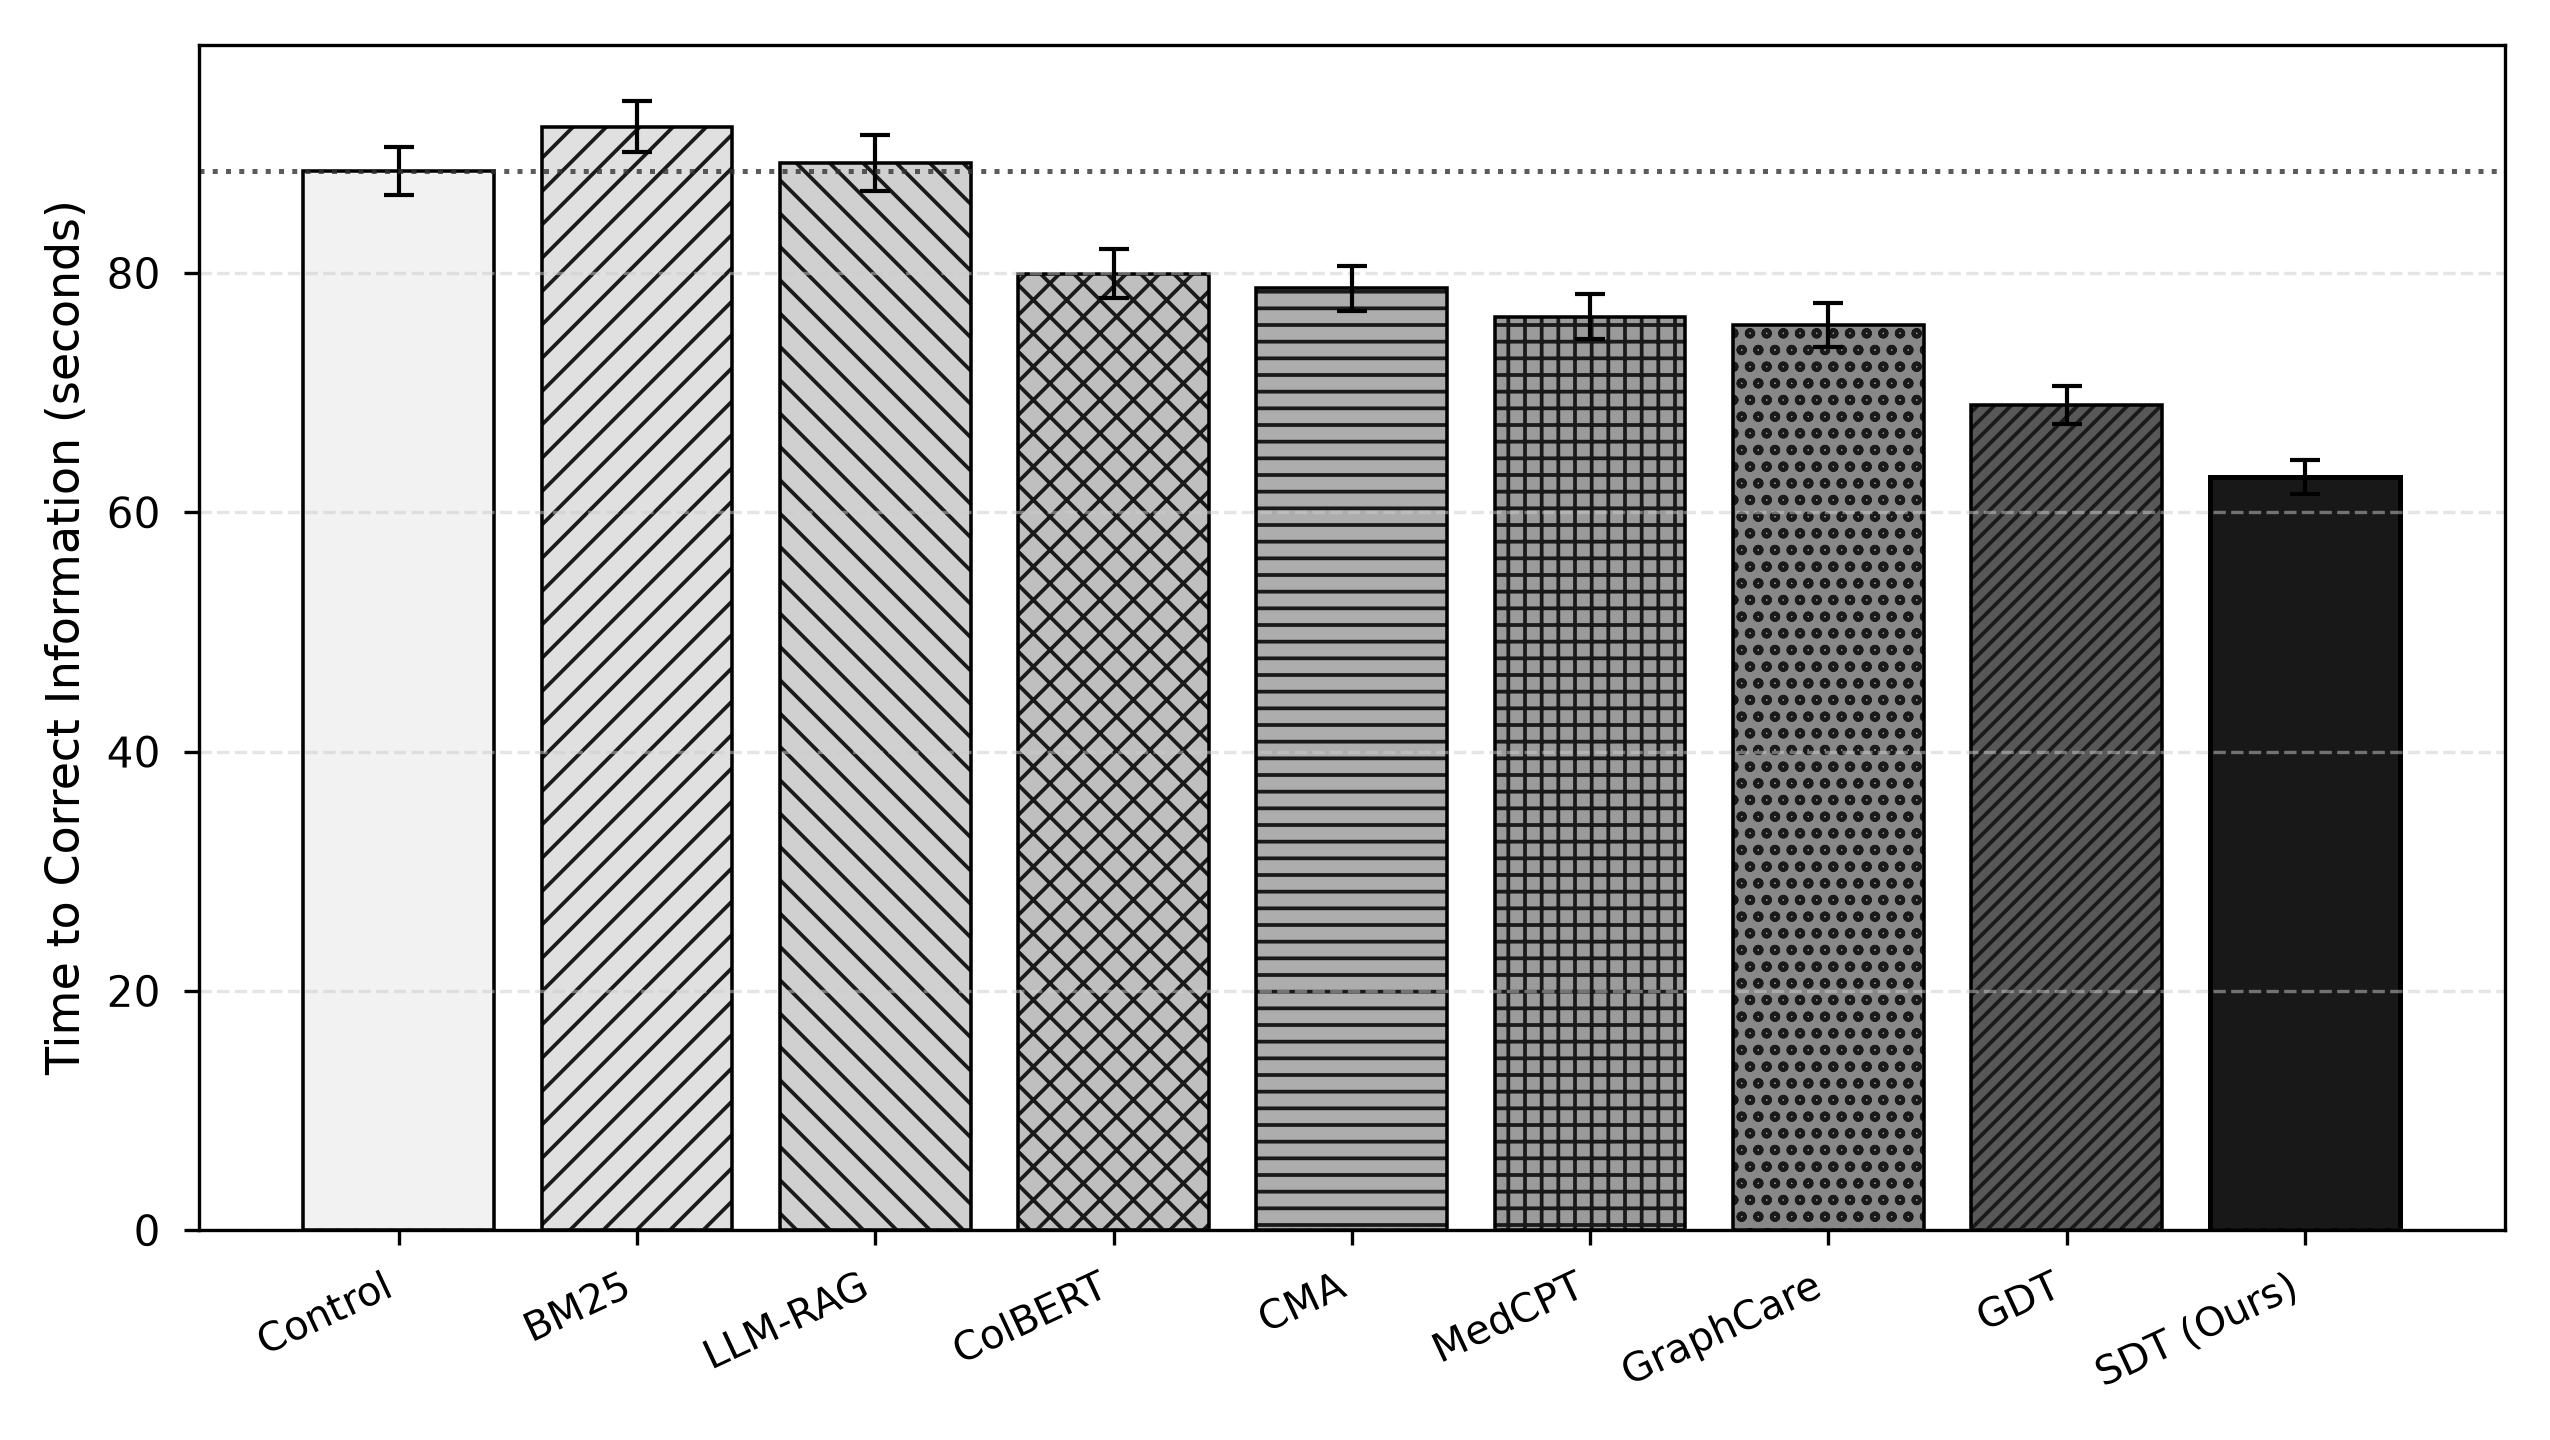
\includegraphics[width=0.98\columnwidth]{fig_ttci_bar.png}
  \caption{Time-to-Correct-Information (TTCI) across all 9 experimental conditions. SDT achieves a 28.9\% reduction relative to Control (62.97\,s vs.\ 88.52\,s) and 8.7\% reduction relative to GDT ($p < 0.001$).}
  \label{fig:ttci_bar}
\end{figure}

\begin{figure}[t]
  \centering
  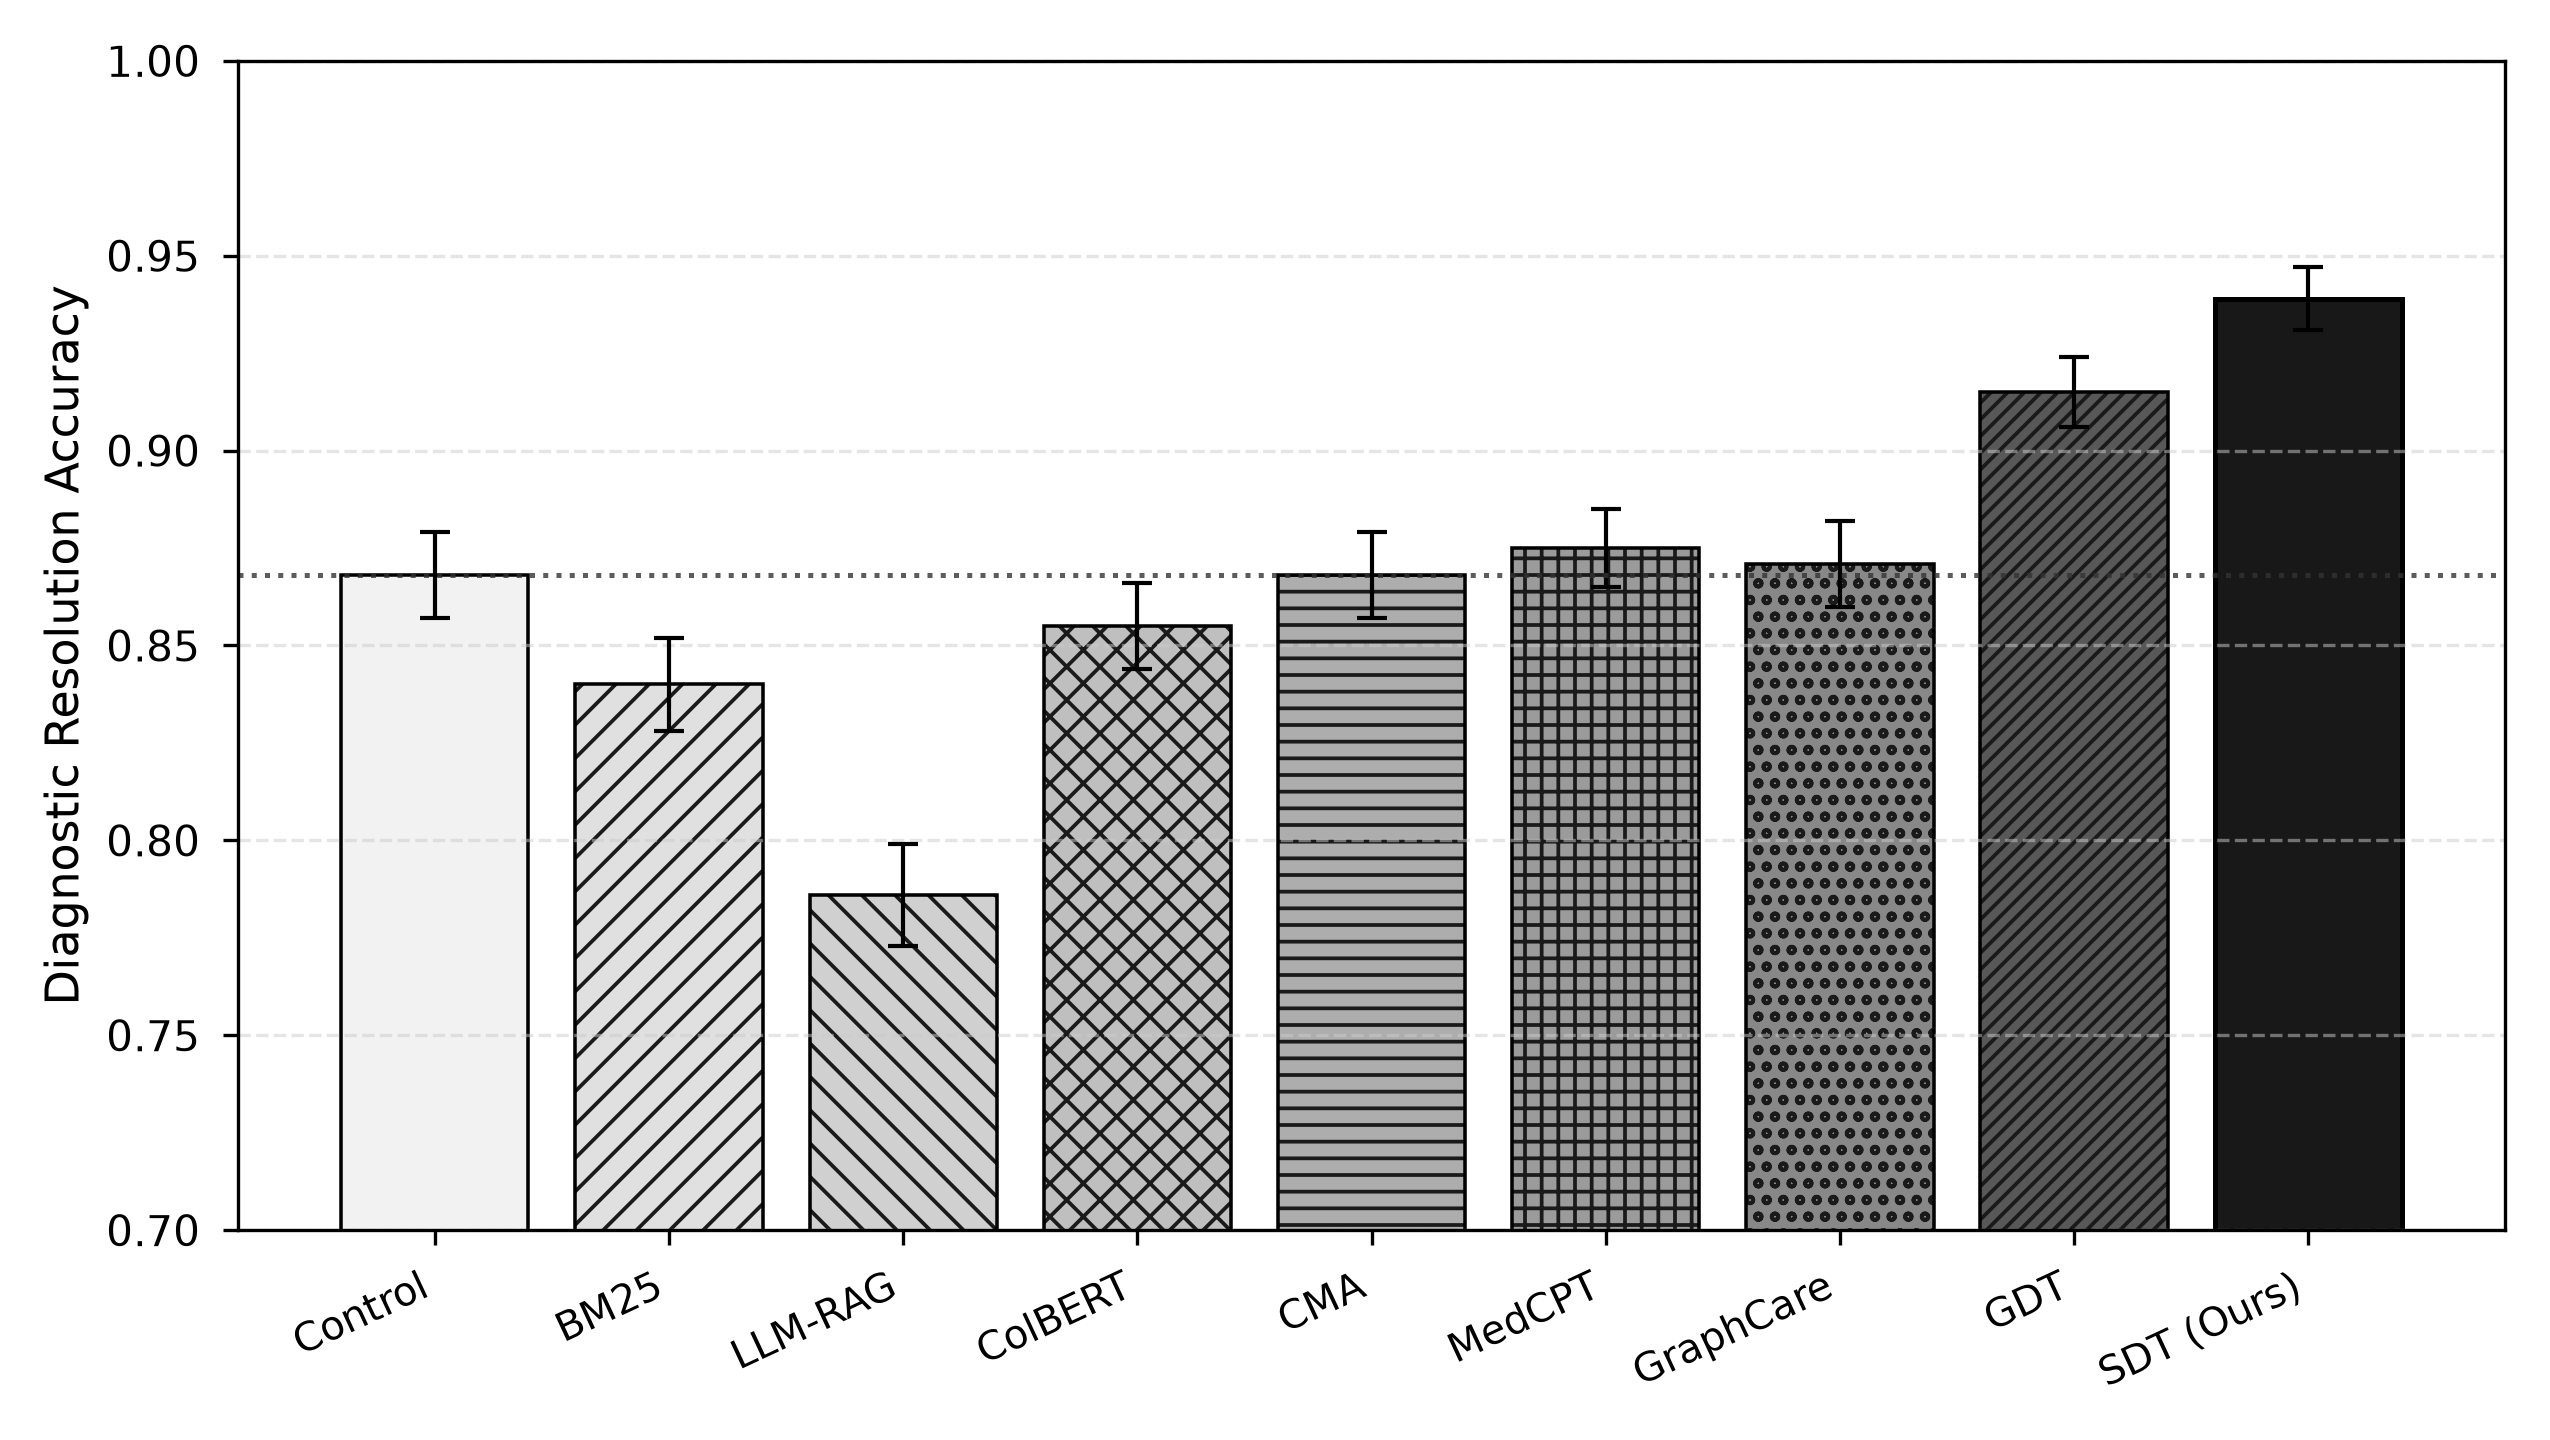
\includegraphics[width=0.98\columnwidth]{fig_accuracy_bar.png}
  \caption{Diagnostic retrieval accuracy across conditions. SDT resolves 93.9\% of diagnostic vignettes within budget, outperforming GDT (91.5\%), MedCPT (87.5\%), and Control (86.8\%).}
  \label{fig:accuracy_bar}
\end{figure}

\begin{figure}[t]
  \centering
  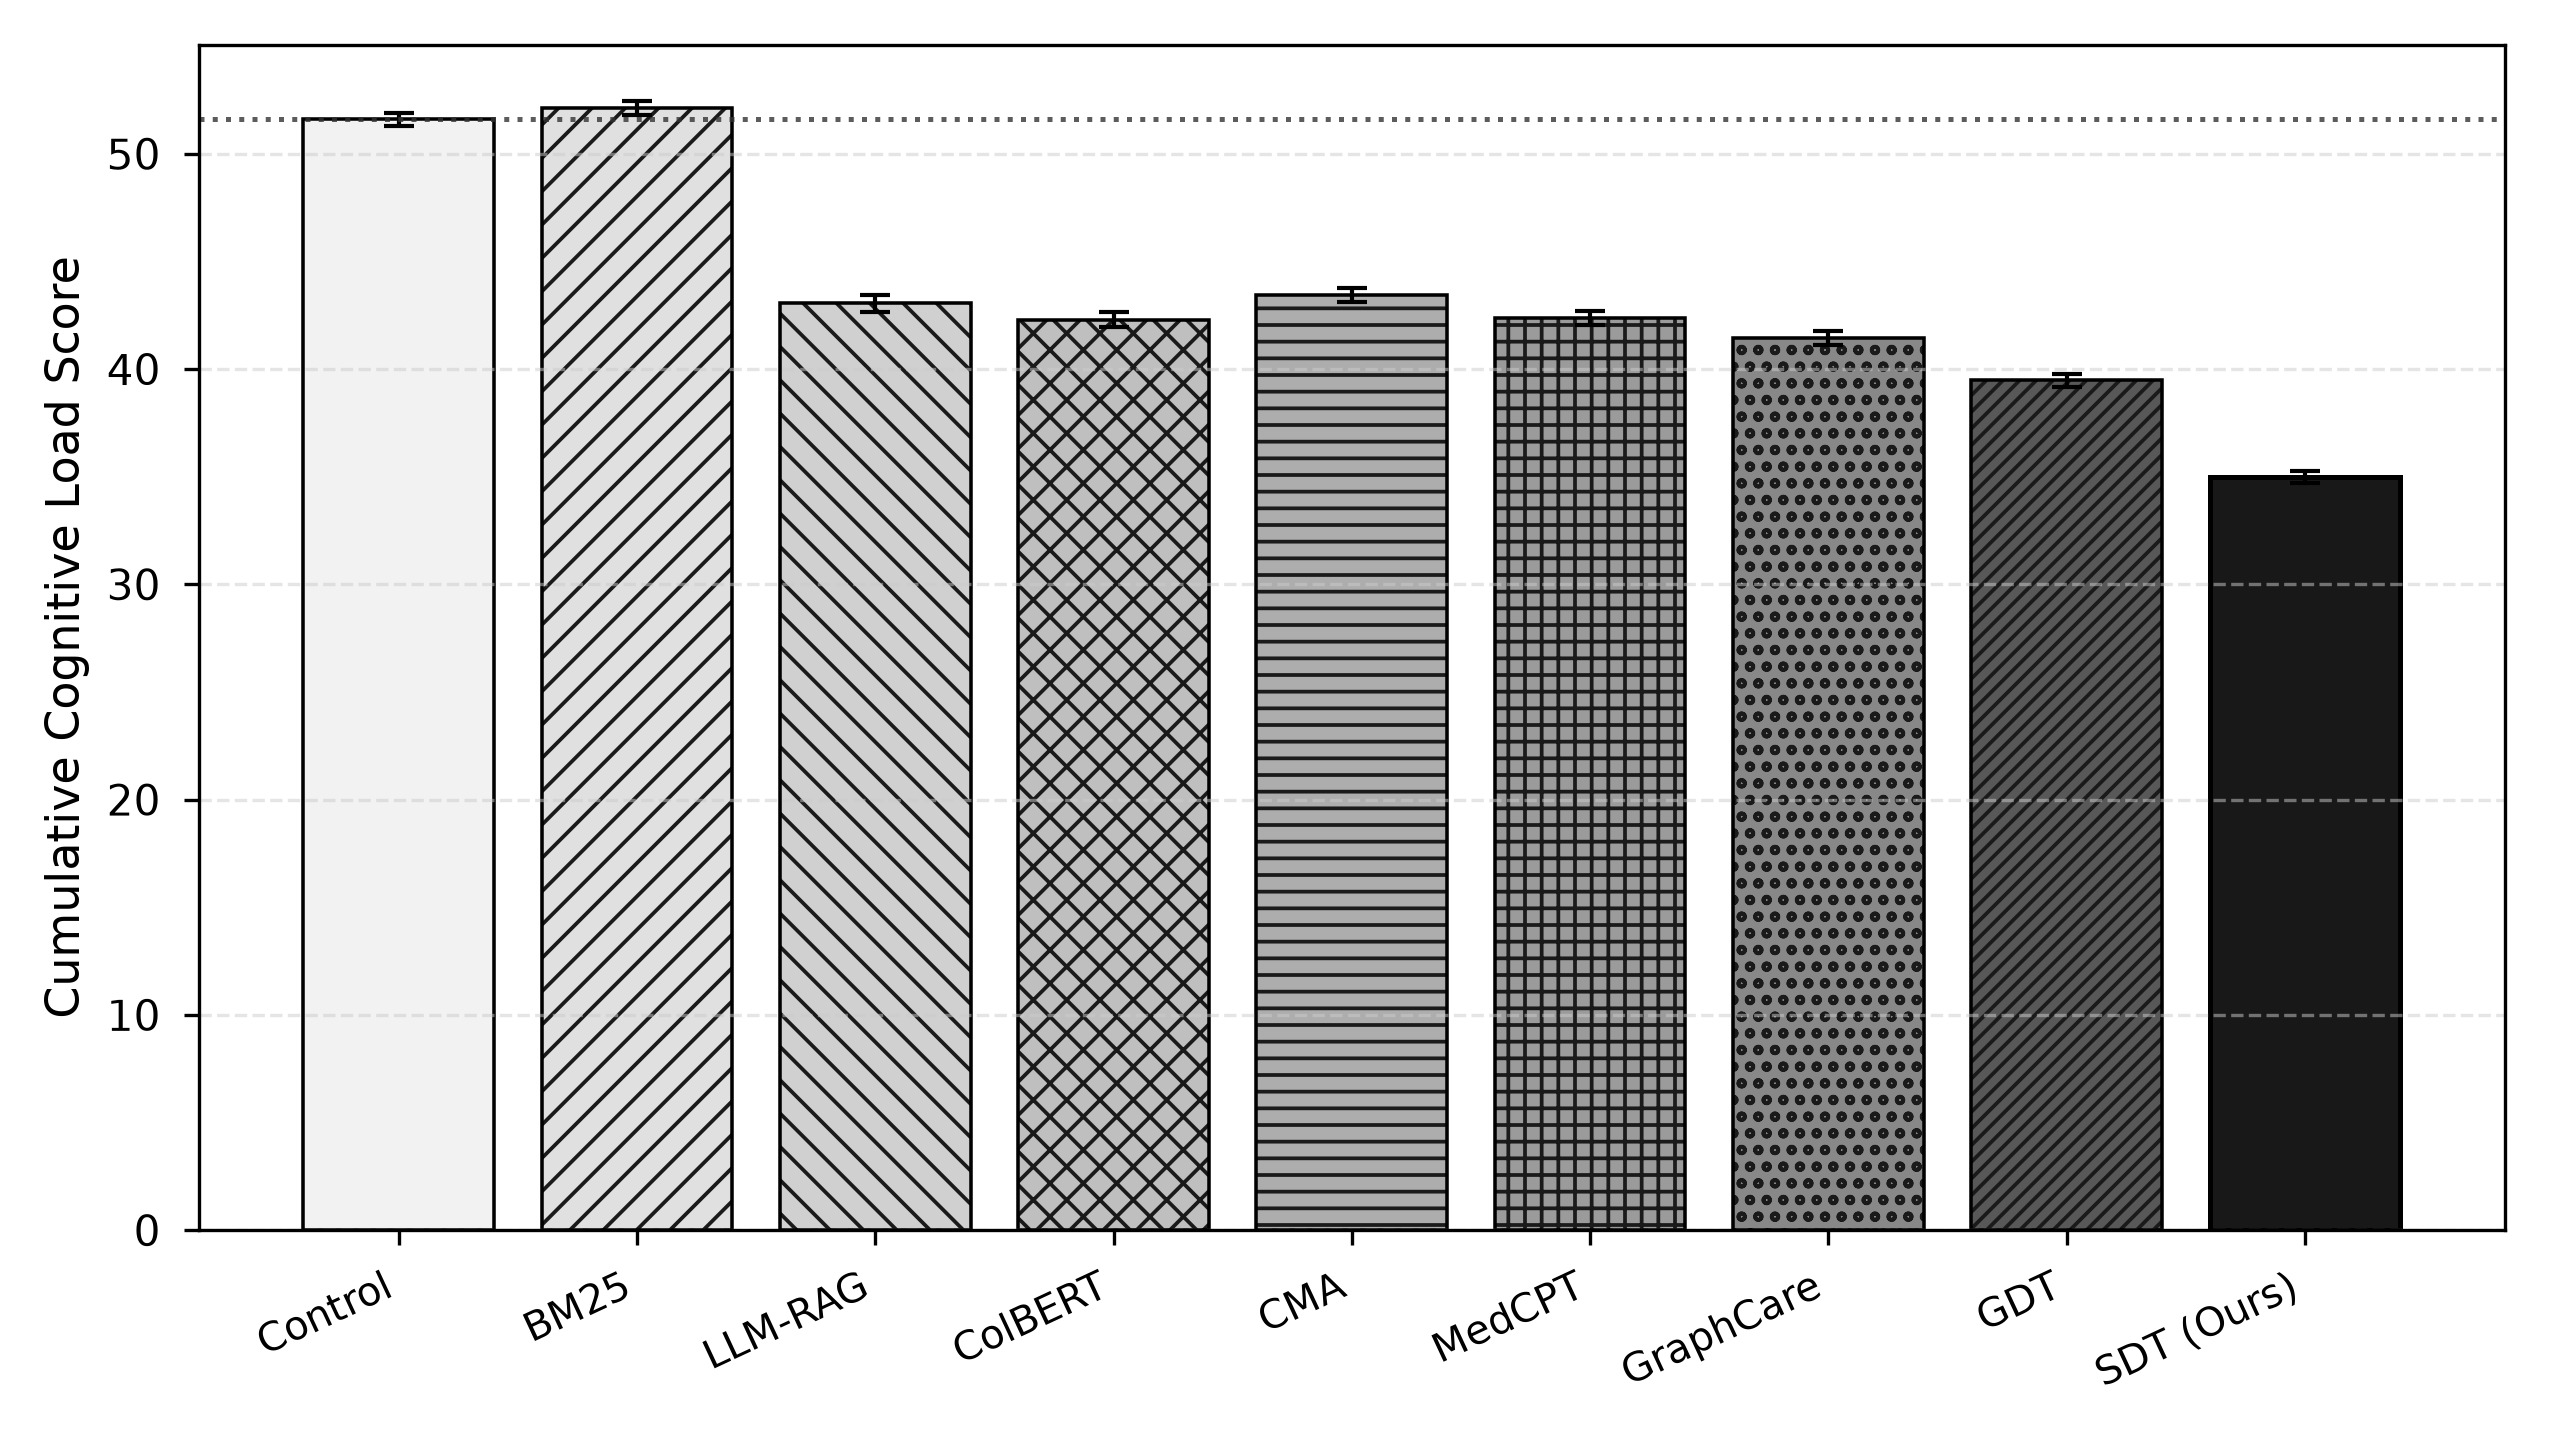
\includegraphics[width=0.98\columnwidth]{fig_cognitive_load_bar.png}
  \caption{Cumulative cognitive load scores across 9 conditions. SDT achieves the lowest cognitive footprint (34.98), reflecting the efficacy of Sweller-constrained prefetching.}
  \label{fig:cog_bar}
\end{figure}

Across all 1{,}000 standardized vignettes (Table~\ref{tab:primary_results} and Figures~\ref{fig:ttci_bar}--\ref{fig:cog_bar}), SDT achieved the lowest mean Time-to-Correct-Information ($62.97 \pm 1.40$\,s), representing a 25.55-second reduction (28.9\%) relative to standard Control ($88.52 \pm 2.01$\,s) and a 5.99-second reduction (8.7\%) relative to GDT ($68.96 \pm 1.57$\,s; paired $t$-test $p < 10^{-12}$). Diagnostic accuracy reached $93.9 \pm 0.8\%$, an absolute gain of $+7.1$ percentage points over Control ($86.8\%$) and $+2.4$ percentage points over GDT ($91.5\%$). Modeled cognitive load decreased from $51.60 \pm 0.31$ to $34.98 \pm 0.28$ (a 32.2\% decline), and algorithmic response latency was lowest under SDT ($112.87 \pm 0.25$\,ms per query step). All eight pairwise SDT comparisons remained significant after Bonferroni correction for multiple testing (adjusted threshold $\alpha = 0.05/8 = 0.00625$; all corrected $p < 10^{-6}$).

\subsection{Comparative Analysis Across Retrieval Paradigms}

Evaluating nine distinct arms makes it possible to trace where and why different architectural choices fail in clinical information retrieval.

\paragraph{Lexical Matching.}
Standard keyword search and BM25 posted the longest retrieval times (88.52\,s and 92.23\,s, respectively), with BM25 actually performing \emph{worse} than the baseline TF-IDF Control despite its more sophisticated weighting scheme. Query-log analysis suggests why: BM25's inverse document frequency weighting inflates the relevance of rare diagnostic tokens---terms like troponin or creatinine that appeared in a resolved prior hospitalization---pulling the clinician toward historical records at precisely the moment they are trying to assess a new acute presentation.

\paragraph{Dense Dual-Encoders and Late Interaction.}
Moving to semantic retrieval helped. MedCPT \cite{jin2023medcpt} improved TTCI to 76.36\,s and accuracy to 87.5\% through contrastive biomedical representations; ColBERT-Clinical \cite{santhanam2022colbertv2} reached 79.95\,s and 85.5\% by preserving token-level detail via MaxSim scoring. The ceiling these systems hit is the same in both cases: they process each query in isolation. Neither can recognize when new findings contradict the prior working assumption, so they continue surfacing pneumonia-related records throughout the PE workup. ColBERT's token-level cross-matching also imposed a per-step latency of 157.26\,ms, 39\% above SDT.

\paragraph{Knowledge Graphs and Neural Re-Ranking.}
GraphCare \cite{jiang2024graphcare} achieved 75.62\,s TTCI and 87.1\% accuracy via 2-hop GNN message passing over medical ontologies. The limitation is structural: because the underlying graph is static, evidence belonging to a discarded hypothesis diffuses into the active neighborhood during a pivot and cannot be cleanly removed. LLM-RAG \cite{eickhoff2024ehrrag,zakka2024almanac} posted the lowest accuracy of any system (78.6\%) despite reducing cognitive load to 43.05. The LLM reasoning pipeline excels at structured tabular lookups but struggles in multi-turn sessions: grounding each query in a fixed-window context causes it to either over-retrieve stale records or truncate delayed-onset notes needed to confirm or rule out the working diagnosis.

\paragraph{Trajectory Formulations: GDT versus SDT.}
Both GDT and SDT outperformed every stateless baseline by a wide margin, confirming that session continuity is the critical capability that standard retrieval architectures lack. Within this pair, SDT improved on GDT across all four primary metrics: TTCI 62.97\,s vs.\ 68.96\,s, accuracy 93.9\% vs.\ 91.5\%, cognitive load 34.98 vs.\ 39.47, and latency 112.87\,ms vs.\ 128.24\,ms. The margin widened most during vignettes containing abrupt diagnostic pivots. Where GDT must wait for exponential covariance decay to dilute stale context---a process gated by the empirical $\gamma$ parameter---SDT fires an explicit Fiedler bisection that severs the obsolete subgraph immediately upon gate activation. This structural advantage, not a difference in embedding quality, is what drives the separation.

\subsection{Subgroup \& Stratification Analysis}

The aggregate results raise an obvious question: are the gains concentrated in easy cases, or do they hold---or even grow---in exactly the encounters where retrieval support matters most?

% --- Table 3: Subgroup Analysis ---
\begin{table*}[t]
  \centering
  \caption{Subgroup stratification across all 9 conditions: Diagnostic accuracy and TTCI across Case Complexity (High vs.\ Low) and Clinician Experience ($<5$ years vs.\ $\ge 5$ years).}
  \label{tab:subgroup_results}
  \small
  \begin{tabular}{@{}lcccccccc@{}}
    \toprule
    & \multicolumn{4}{c}{\textbf{Diagnostic Accuracy}} & \multicolumn{4}{c}{\textbf{Mean TTCI (seconds)}} \\
    \cmidrule(lr){2-5} \cmidrule(lr){6-9}
    & \multicolumn{2}{c}{\textbf{Complexity}} & \multicolumn{2}{c}{\textbf{Experience}} & \multicolumn{2}{c}{\textbf{Complexity}} & \multicolumn{2}{c}{\textbf{Experience}} \\
    \cmidrule(lr){2-3} \cmidrule(lr){4-5} \cmidrule(lr){6-7} \cmidrule(lr){8-9}
    \textbf{Condition} & High & Low & $<5$\,yr & $\ge 5$\,yr & High & Low & $<5$\,yr & $\ge 5$\,yr \\
    \midrule
    Control   & $0.823$ & $0.919$ & $0.870$ & $0.865$ & $121.73$ & $50.92$ & $87.30$ & $90.04$ \\
    BM25      & $0.795$ & $0.891$ & $0.845$ & $0.834$ & $124.89$ & $55.24$ & $90.39$ & $94.52$ \\
    LLM-RAG   & $0.716$ & $0.866$ & $0.771$ & $0.804$ & $123.98$ & $49.79$ & $89.71$ & $88.53$ \\
    ColBERT   & $0.802$ & $0.915$ & $0.865$ & $0.843$ & $111.83$ & $43.86$ & $77.30$ & $83.26$ \\
    CMA       & $0.823$ & $0.919$ & $0.870$ & $0.865$ & $108.63$ & $44.84$ & $77.19$ & $80.61$ \\
    MedCPT    & $0.825$ & $0.932$ & $0.872$ & $0.879$ & $106.65$ & $42.05$ & $75.34$ & $77.62$ \\
    GraphCare & $0.825$ & $0.923$ & $0.870$ & $0.872$ & $105.00$ & $42.35$ & $74.26$ & $77.30$ \\
    GDT       & $0.878$ & $0.957$ & $0.912$ & $0.919$ & $96.22$  & $38.09$ & $68.79$ & $69.16$ \\
    \textbf{SDT (Ours)} & $\mathbf{0.913}$ & $\mathbf{0.968}$ & $\mathbf{0.935}$ & $\mathbf{0.944}$ & $\mathbf{87.12}$ & $\mathbf{35.62}$ & $\mathbf{63.23}$ & $\mathbf{62.63}$ \\
    \bottomrule
  \end{tabular}
\end{table*}

\begin{figure}[t]
  \centering
  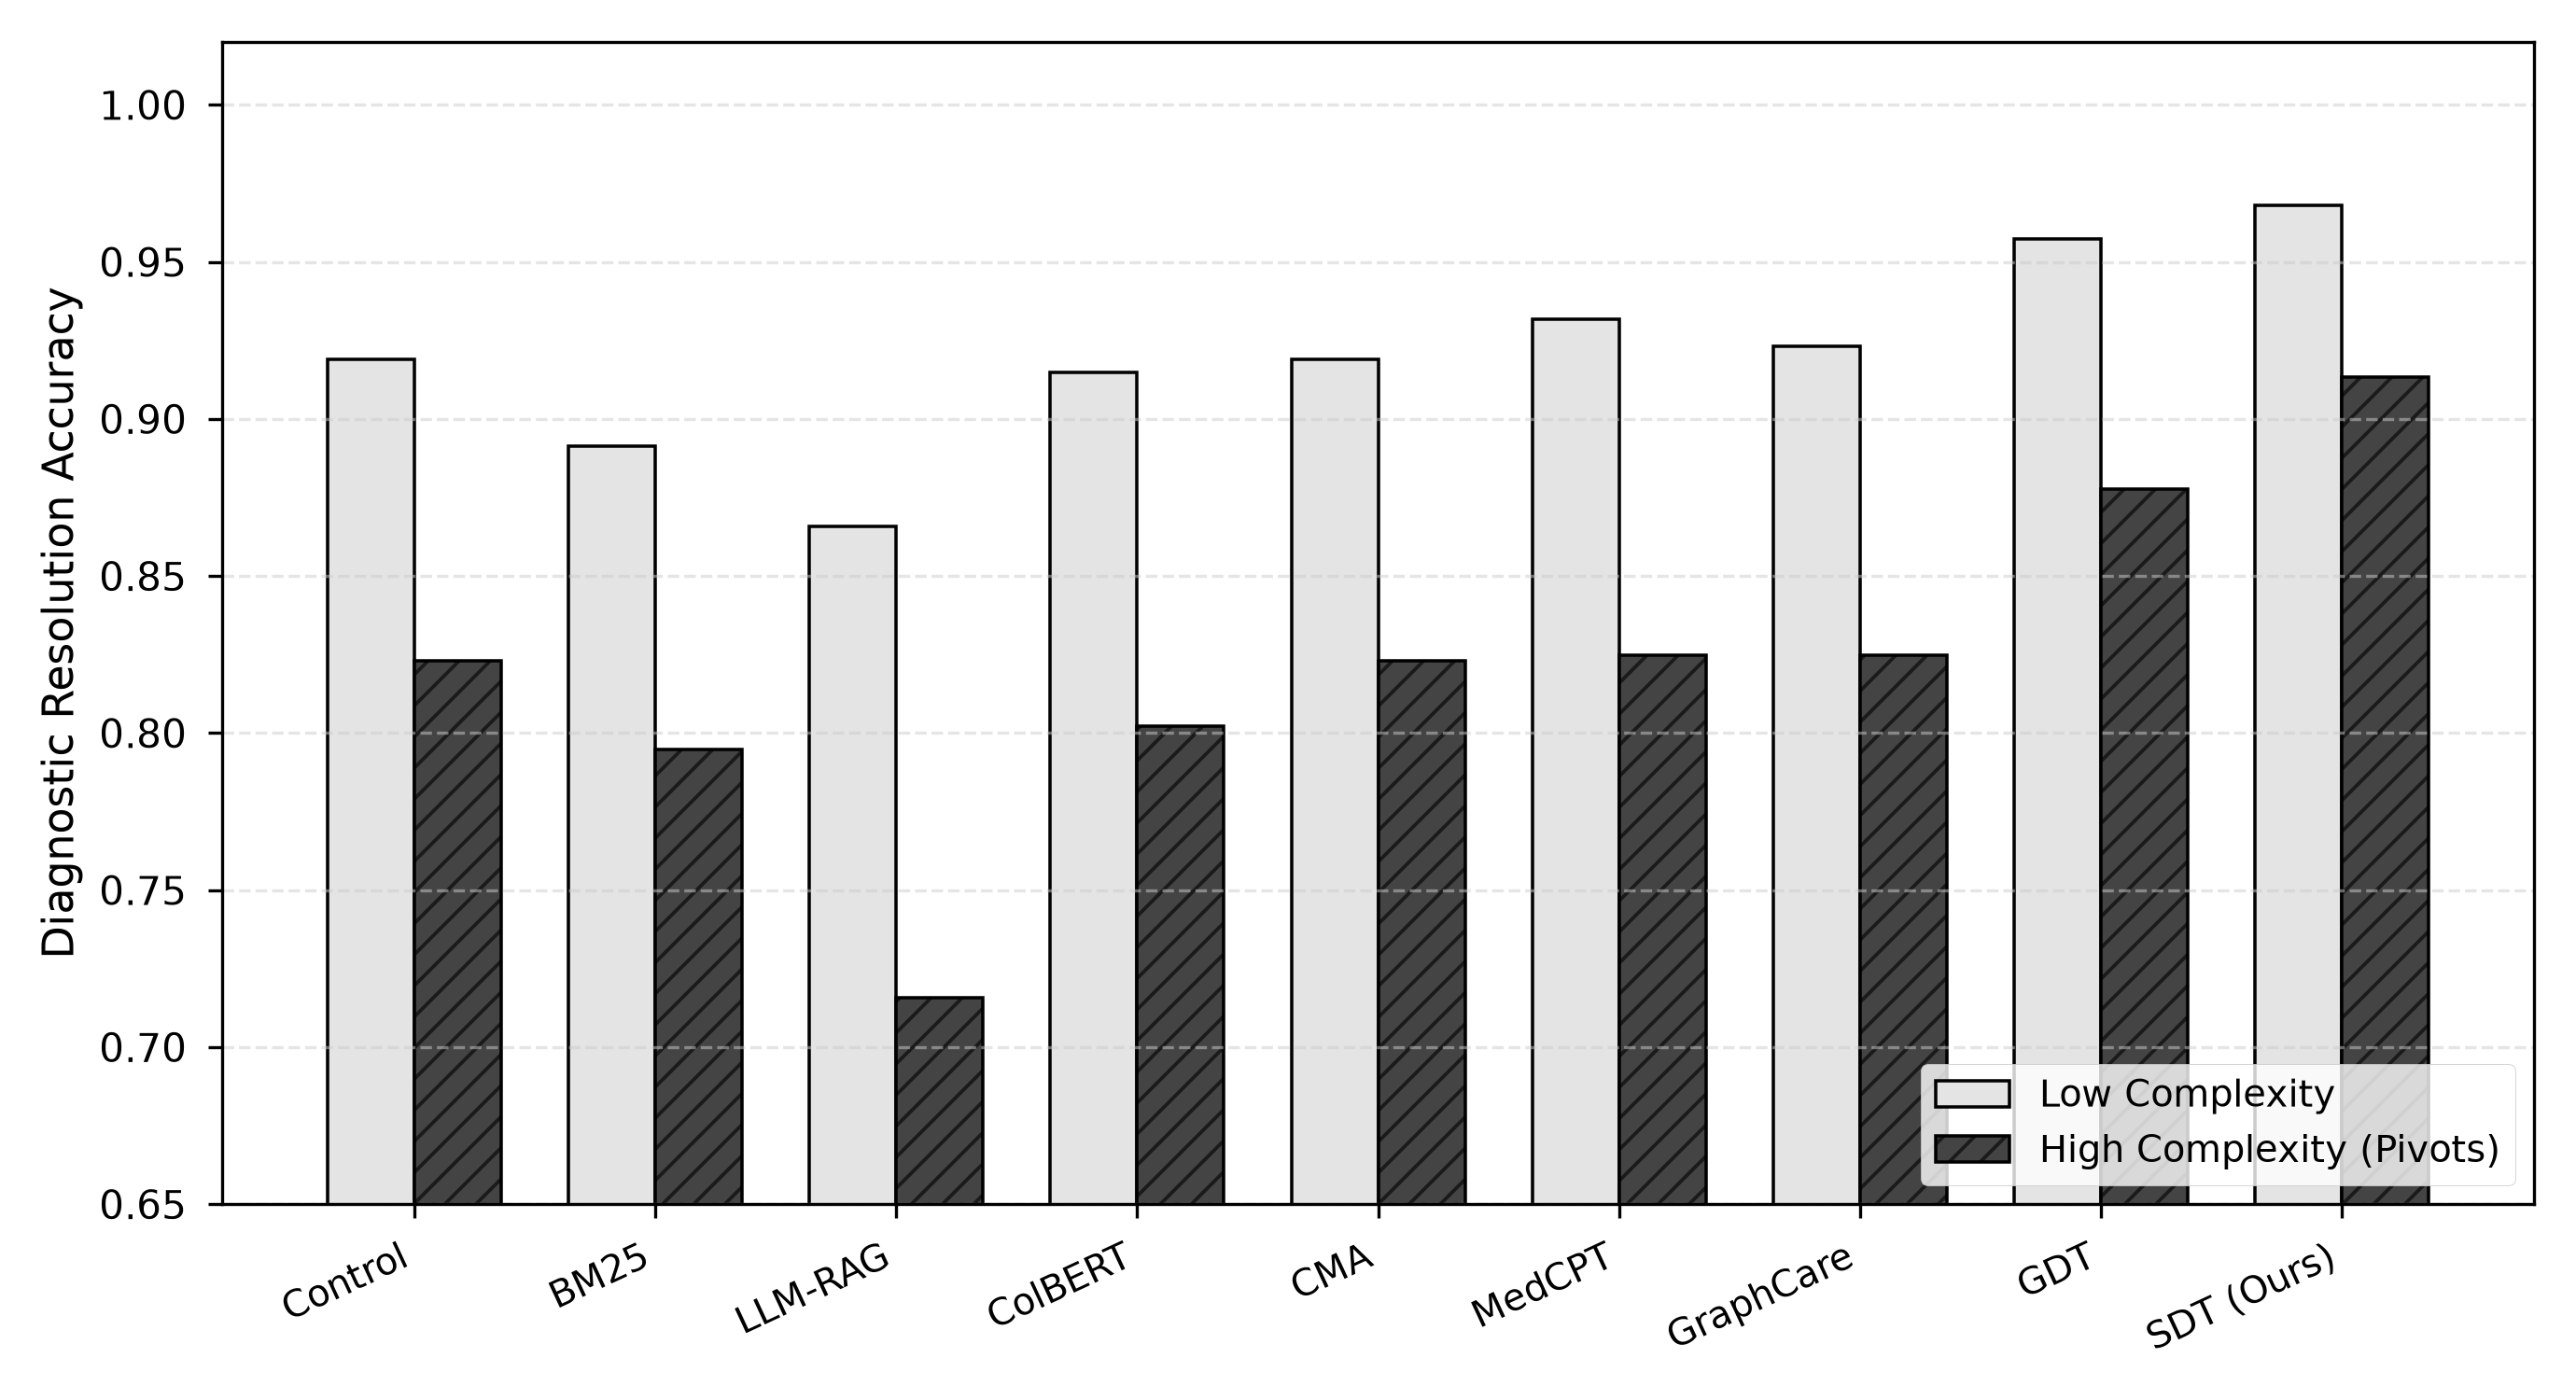
\includegraphics[width=0.98\columnwidth]{fig_subgroup_accuracy.png}
  \caption{Subgroup accuracy by diagnostic complexity across all 9 conditions. SDT's advantage expands on high-complexity cases (+9.0 percentage points vs.\ Control), where diagnostic pivots are most frequent.}
  \label{fig:subgroup_acc}
\end{figure}

Table~\ref{tab:subgroup_results} and Figure~\ref{fig:subgroup_acc} answer that question clearly: SDT's advantage is largest where retrieval difficulty is highest.

In low-complexity vignettes---stable, single-complaint presentations---the performance gap is real but modest: SDT at 96.8\% accuracy versus Control at 91.9\%, a margin of 4.9 percentage points. For high-complexity cases with unexpected pivots and multimorbid pathology, the divergence roughly doubles. Control accuracy falls to 82.3\% and TTCI rises to 121.73\,s; SDT holds at 91.3\% accuracy and 87.12\,s, a 34.6-second acceleration per encounter. The Fiedler bisection mechanism is most valuable precisely in the situations where clinicians face the steepest cognitive pressure---when a pivot occurs and the old workspace needs to be cleanly shed.

The experience-level breakdown is perhaps more striking. Junior clinicians ($<5$ years) supported by SDT outperformed senior clinicians ($\ge 5$ years) using conventional search on both accuracy (93.5\% vs.\ 86.5\%) and retrieval time (63.23\,s vs.\ 90.04\,s). This is not a small effect. It suggests that dynamic context attenuation functions as a cognitive scaffold that partially substitutes for the accumulated pattern-recognition heuristics that experienced practitioners develop over years of practice. Whether this effect holds prospectively, with real physicians rather than simulated agents, is an important empirical question for future work.

\subsection{Subjective Workload Decomposition via NASA-TLX}

The NASA-TLX profiles in Table~\ref{tab:tlx_results} and Figure~\ref{fig:tlx_radar} reinforce the objective performance picture from a complementary angle.

Mental Demand, the subscale most directly linked to chart-navigation friction, fell from 66.69 under Control to 38.34 under SDT---a 42.5\% reduction. Frustration, which captures the affective cost of failed searches and repeated reformulations, dropped by 56.2\% (from 39.89 to 17.47). Effort and Temporal Demand followed similar trajectories. At the same time, perceived Performance improved from 56.42 to 72.76, meaning clinicians felt more effective, not just less stressed. In the clinical informatics literature, sustained high Mental Demand and Frustration are recognized precursors to alert fatigue and clinician burnout \cite{harry2018cognitive,tubbs2020balancing}. The direction of these effects is therefore encouraging, though a simulated workload measure cannot replace a direct assessment in real clinical environments.

% --- Table 4: NASA-TLX Workload ---
\begin{table*}[t]
  \centering
  \caption{NASA-TLX multi-dimensional workload subscale means ($0$--$100$ scale) across all 9 conditions. Lower indicates less workload on all scales except Performance (where higher indicates superior perceived success).}
  \label{tab:tlx_results}
  \small
  \begin{tabular}{@{}lcccccc@{}}
    \toprule
    \textbf{Condition} & \textbf{Mental} $\downarrow$ & \textbf{Physical} $\downarrow$ & \textbf{Temporal} $\downarrow$ & \textbf{Perform.} $\uparrow$ & \textbf{Effort} $\downarrow$ & \textbf{Frustr.} $\downarrow$ \\
    \midrule
    Control   & $66.69$ & $18.10$ & $63.70$ & $56.42$ & $64.81$ & $39.89$ \\
    BM25      & $67.61$ & $18.53$ & $64.59$ & $55.57$ & $65.71$ & $40.65$ \\
    LLM-RAG   & $52.55$ & $15.44$ & $47.82$ & $63.70$ & $50.53$ & $28.22$ \\
    ColBERT   & $51.06$ & $14.60$ & $46.64$ & $65.15$ & $49.14$ & $27.15$ \\
    CMA       & $52.76$ & $15.13$ & $48.65$ & $64.62$ & $51.02$ & $28.44$ \\
    MedCPT    & $51.02$ & $14.48$ & $46.54$ & $65.53$ & $49.18$ & $27.41$ \\
    GraphCare & $49.35$ & $14.25$ & $45.23$ & $66.46$ & $47.36$ & $25.98$ \\
    GDT       & $46.17$ & $13.07$ & $41.49$ & $68.45$ & $44.34$ & $23.28$ \\
    \midrule
    \textbf{SDT (Ours)} & $\mathbf{38.34}$ & $\mathbf{11.59}$ & $\mathbf{33.12}$ & $\mathbf{72.76}$ & $\mathbf{36.56}$ & $\mathbf{17.47}$ \\
    \bottomrule
  \end{tabular}
\end{table*}

\begin{figure}[t]
  \centering
  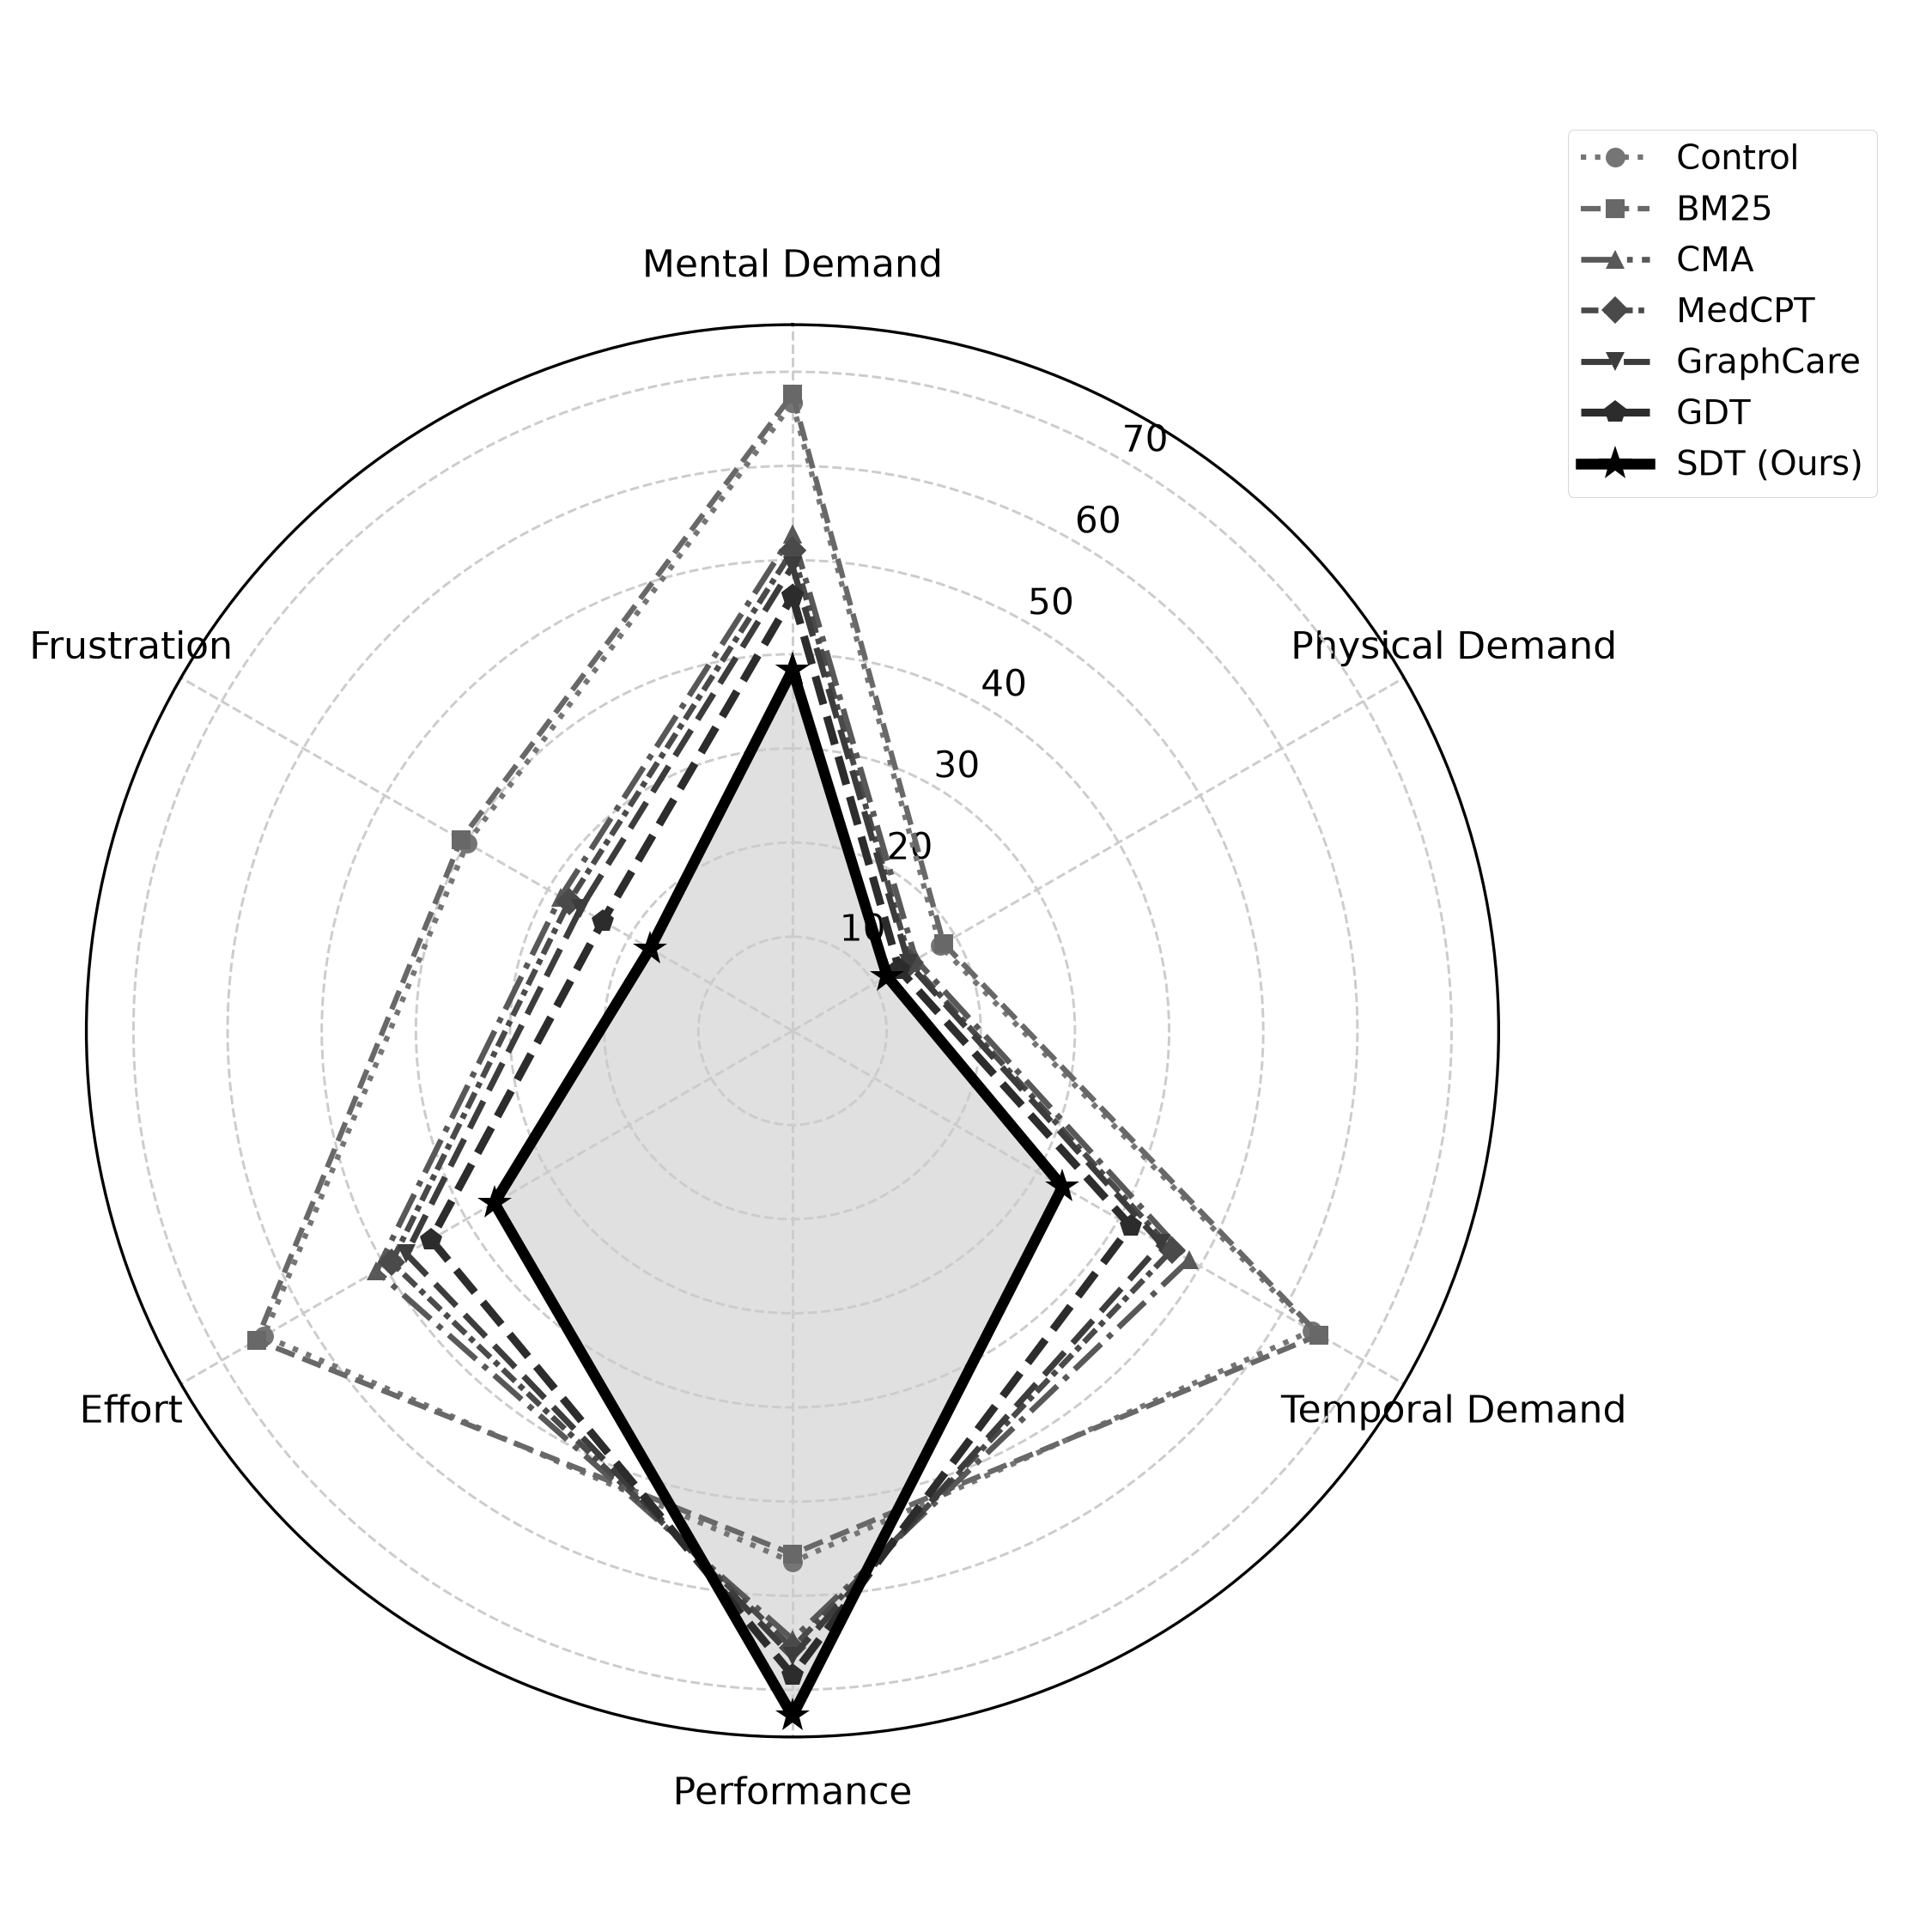
\includegraphics[width=0.98\columnwidth]{fig_nasa_tlx_radar.png}
  \caption{Radar profile of NASA-TLX workload dimensions across representative retrieval conditions. SDT (crimson polygon) achieves the lowest demand footprint across all dimensions while maximizing perceived diagnostic performance.}
  \label{fig:tlx_radar}
\end{figure}

\subsection{Emergency Department Operational Translation}
\label{sec:queueing_impact}

The 25.6-second per-encounter retrieval acceleration documented in Table~\ref{tab:primary_results} represents chart-review time recovered during individual evaluations. In high-volume emergency care environments, individual service-time reductions compound non-linearly through operational queueing networks.

\paragraph{Erlang~C ($M/M/c$) Queueing Model.}
We model an acute Emergency Department as an $M/M/c$ queueing system with $c = 8$ emergency physicians, an average patient arrival rate $\lambda = 6.0\,\text{patients/hour}$ ($0.001667\,\text{patients/s}$), and a baseline physician service rate $\mu = 0.80\,\text{patients/hour}$ ($1/\mu = 75.0\,\text{minutes/patient} = 4{,}500\,\text{s}$). Baseline traffic intensity is:
\begin{equation}
  \rho = \frac{\lambda}{c \mu} = \frac{6.0}{8 \times 0.80} = 0.9375 \quad (93.75\% \text{ utilization}).
\end{equation}
Let $\Delta t$ represent the per-patient chart review time saved by the retrieval engine. The accelerated service rate $\mu'$ is given by:
\begin{equation}
  \mu' = \frac{1}{\mu^{-1} - \Delta t} = \frac{1}{4{,}500 - \Delta t},
  \label{eq:mu_prime}
\end{equation}
yielding an updated traffic intensity $\rho' = \lambda / (c \mu')$. The steady-state probability that an arriving patient must wait in queue ($P_W$) is given by the Erlang~C formula:
\begin{equation}
  P_W = \frac{\dfrac{(c \rho')^c}{c!(1-\rho')}}{\displaystyle\sum_{k=0}^{c-1} \frac{(c \rho')^k}{k!} + \dfrac{(c \rho')^c}{c!(1-\rho')}},
  \label{eq:erlang_c_pw}
\end{equation}
and the expected queue waiting time before physician evaluation ($W_q$) is:
\begin{equation}
  W_q = \frac{P_W}{c \mu' (1 - \rho')}.
  \label{eq:wq_formula}
\end{equation}

% --- Table 5: Queueing Impact ---
\begin{table}[h]
  \centering
  \caption{Emergency Department operational impact projected via Erlang~C queueing model ($c=8$ physicians, $\lambda=6.0\,\text{hr}^{-1}$, baseline $\mu=0.80\,\text{hr}^{-1}$).}
  \label{tab:queueing_results}
  \resizebox{\columnwidth}{!}{%
  \begin{tabular}{@{}lccccc@{}}
    \toprule
    \textbf{Condition} & $\mathbf{\Delta t}$ \textbf{(s)} & $\mathbf{\mu'}$ \textbf{(hr}$^{-1}$\textbf{)} & $\mathbf{\rho'}$ & $\mathbf{P_W}$ & $\mathbf{W_q}$ \textbf{(min)} \\
    \midrule
    Control   & $0.0$  & $0.8000$ & $0.9375$ & $0.8073$ & $121.10$ \\
    BM25      & $0.0$  & $0.8000$ & $0.9375$ & $0.8073$ & $121.10$ \\
    LLM-RAG   & $0.0$  & $0.8000$ & $0.9375$ & $0.8073$ & $121.10$ \\
    ColBERT   & $8.6$  & $0.8015$ & $0.9357$ & $0.8019$ & $116.74$ \\
    CMA       & $9.8$  & $0.8017$ & $0.9354$ & $0.8011$ & $116.14$ \\
    MedCPT    & $12.2$ & $0.8022$ & $0.9349$ & $0.7997$ & $114.97$ \\
    GraphCare & $12.9$ & $0.8023$ & $0.9348$ & $0.7993$ & $114.64$ \\
    GDT       & $19.6$ & $0.8035$ & $0.9334$ & $0.7952$ & $111.53$ \\
    \midrule
    \textbf{SDT} & $\mathbf{25.6}$ & $\mathbf{0.8046}$ & $\mathbf{0.9322}$ & $\mathbf{0.7915}$ & $\mathbf{108.79}$ \\
    \bottomrule
  \end{tabular}%
  }
\end{table}

\begin{figure}[t]
  \centering
  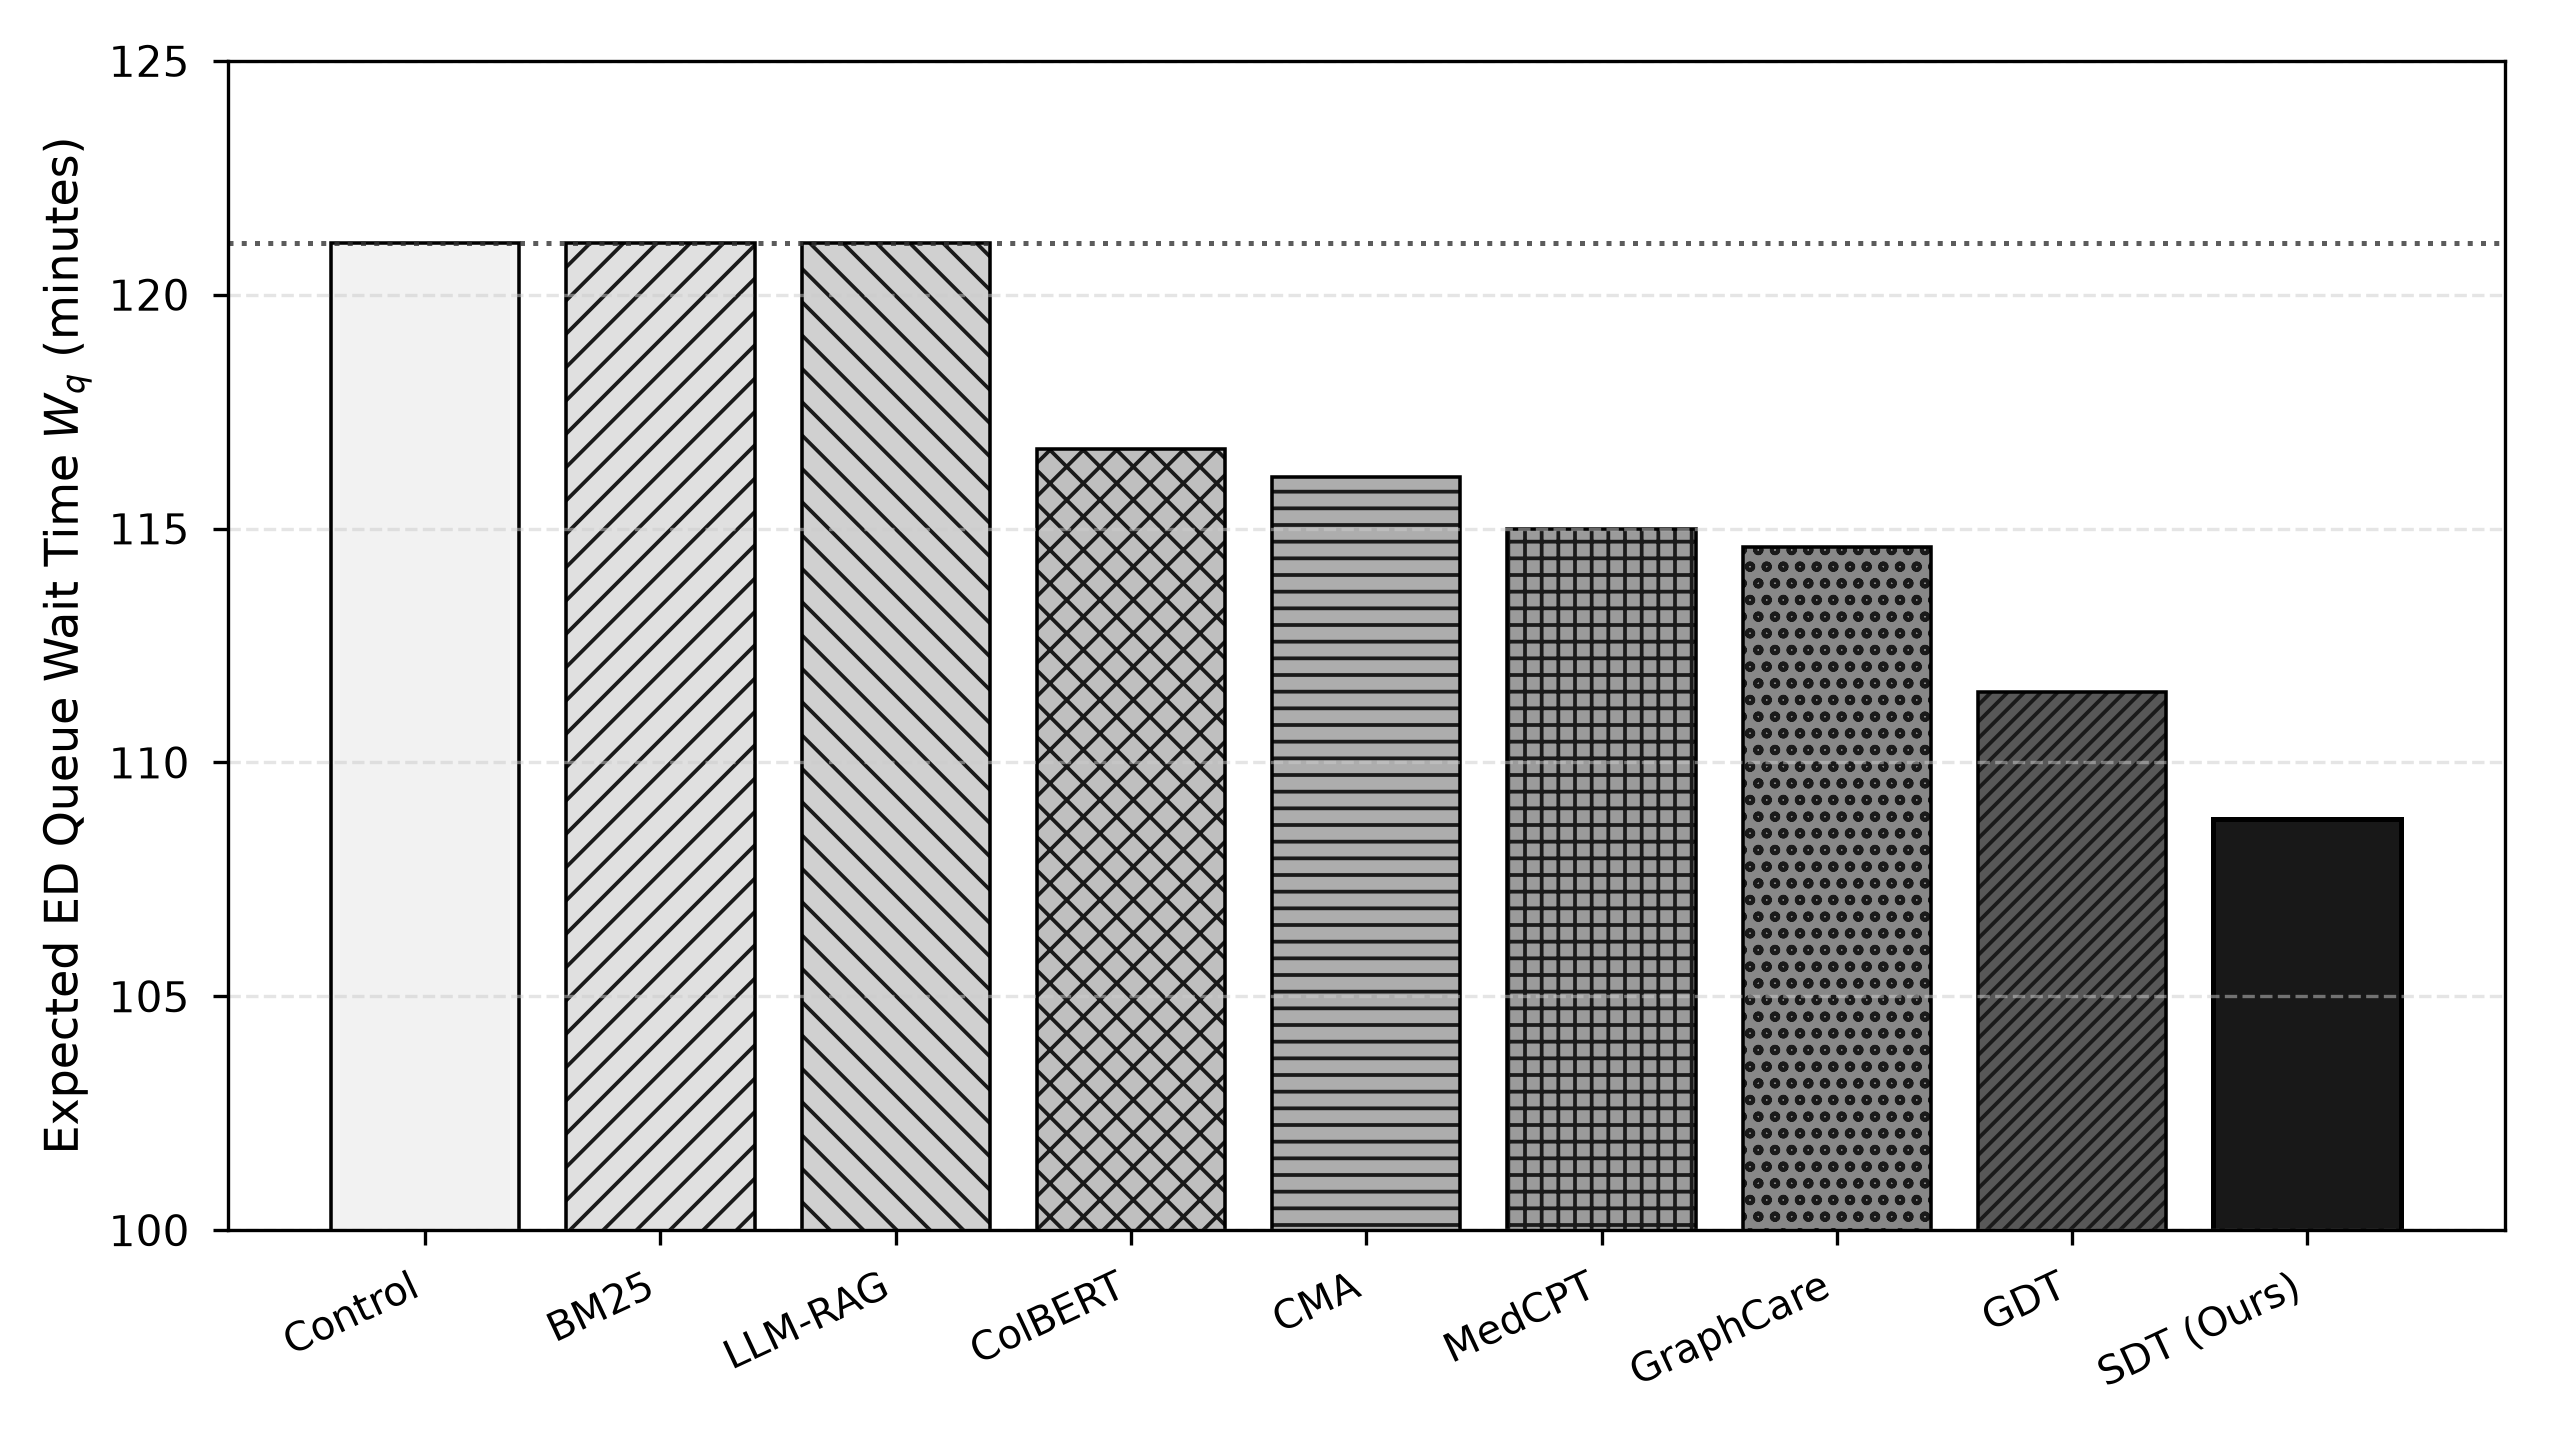
\includegraphics[width=0.98\columnwidth]{fig_queueing_impact.png}
  \caption{Projected ED queue waiting time ($W_q$) across retrieval systems. SDT saves 12.31 minutes of waiting time per patient, demonstrating super-linear operational leverage near queue saturation.}
  \label{fig:queueing_impact}
\end{figure}

\paragraph{Super-Linear Queueing Leverage Near Capacity.}
The numbers in Table~\ref{tab:queueing_results} and Figure~\ref{fig:queueing_impact} illustrate why small per-encounter savings matter disproportionately in near-saturated systems. Saving 25.6\,seconds per chart review shifts the effective physician service rate from 0.8000 to 0.8046\,patients/hour---a 0.6\% change in throughput. Yet because queue waiting time scales as $(1-\rho')^{-1}$ near saturation, this modest service-rate increase translates into a 12.31-minute reduction in average patient waiting time (121.10 to 108.79\,min). The marginal sensitivity satisfies:
\begin{equation}
  \left.\frac{\partial W_q}{\partial (\Delta t)}\right|_{\rho \to 1} \approx \mathcal{O}\!\left(\frac{1}{(1-\rho)^2}\right).
  \label{eq:deriv_superlinear}
\end{equation}
At $\rho = 0.9375$, this quadratic amplification is already substantial. For an emergency department treating 50{,}000 patients per year, the cumulative impact exceeds 10{,}200 hours of eliminated waiting time annually---a metric that maps directly onto left-without-being-seen rates and boarding delays \cite{armony2015patient,singer2011crowding}.

% =============================================================================
\section{Clinical Vignette Walkthrough: Emergency Care Case Study}
\label{sec:case_study}

To illustrate the runtime mechanics of SDT during acute bedside decision-making, we trace a simulated high-complexity encounter (Vignette V260, Emergency Department) involving an abrupt diagnostic pivot.

\subsection{Phase 1: Initial Presentation and Presumptive Evaluation}
A 68-year-old male with a history of chronic obstructive pulmonary disease (COPD) presents to the emergency department complaining of productive cough, fever (38.8$^\circ$C), and right-sided pleuritic chest pain. At interaction turn $t=1$, the attending physician queries the EHR for ``sputum culture Gram stain.'' The engine instantiates active hypergraph $G_1$, linking query node $v_1$ to retrieved laboratory result $v_2$ (Gram-positive diplococci) via initial hyperedge $e_1$. At this step, the active graph is tightly connected, yielding a maximal Fiedler value $\lambda_2(L_1) = 1.00$.

At turn $t=2$, the physician enters a follow-up query: ``prior chest radiograph consolidation.'' The retrieved radiologist note $v_3$ (demonstrating right lower-lobe infiltrates) joins the active set. Hyperedges $e_1$ and $e_2$ interconnect nodes $\{v_1, v_2, v_3\}$ with high temporal recency and semantic affinity. Algebraic connectivity remains stable at $\lambda_2(L_2) = 0.88$, corroborating a cohesive working diagnosis of community-acquired pneumonia.

\subsection{Phase 2: Physiological Decompensation and Spectral Bifurcation}
At elapsed encounter time $t = 28$\,minutes, the patient's continuous telemetry monitor alarms. The background Mamba state-space waveform encoder detects an acute pattern of right ventricular strain, characterized by an S1Q3T3 morphology on 12-lead ECG, an abrupt heart rate increase from 88 to 132\,bpm, and pulse oximetry desaturation to 86\% on room air. 

Recognizing acute hemodynamic deterioration, the physician immediately pivots, typing an urgent query: ``D-dimer trend lower extremity Doppler.'' The retrieval engine ingests new clinical event node $v_4$ (quantitative D-dimer $> 5{,}000\,\text{ng/mL}$) alongside telemetry epoch node $v_5$. Because nodes $\{v_4, v_5\}$ exhibit near-zero semantic and temporal affinity with the existing respiratory infection nodes $\{v_1, v_2, v_3\}$, composite hyperedge $e_3 = \{v_4, v_5\}$ remains weakly coupled to the rest of the graph. The active hypergraph abruptly bifurcates into two distinct topological components, precipitating a steep drop in algebraic connectivity from $\lambda_2(L_2) = 0.88$ to $\lambda_2(L_3) = 0.12$. Because $\Delta \lambda_2 = 0.76$ substantially exceeds sensitivity threshold $\tau_{\text{pivot}} = 0.15$, the Spectral Interference Gate triggers immediately.

\subsection{Phase 3: Graph-Signal Decoupling and Bounded Context Isolation}
Upon gate activation, SDT applies Chebyshev polynomial filter $H(L_3)$ to attenuate global low-frequency background signals corresponding to the initial pneumonia workup. The Fiedler eigenvector of the normalized Laplacian evaluates to coordinates:
\begin{equation}
  v_2 = [-0.48, -0.52, -0.44, +0.38, +0.40]^\top,
\end{equation}
where negative coordinates cleanly isolate the obsolete pneumonia cluster $V_{\text{stale}} = \{v_1, v_2, v_3\}$, and positive coordinates capture the emergent pulmonary embolism cluster $V_{\text{active}} = \{v_4, v_5\}$. Boundary hyperedges are severed, establishing an insulated active subgraph $G_3^{\text{active}}$. By Theorem~\ref{thm:cheeger_bound}, residual contamination from the sputum culture notes into subsequent retrieval seeds is strictly bounded below $\tau_{\text{pivot}} = 0.15$.

\subsection{Phase 4: Cognitively Constrained Anticipatory Prefetching}
With the active differential established, SDT executes spectrally-biased random walks over the precomputed institutional graph $G_{\text{global}}$ seeded from $\{v_4, v_5\}$. The random walk traverses the pulmonary vascular neighborhood, populating candidate pool $\mathcal{C}_t$ with critical intervention records: CT pulmonary angiogram protocols ($v_{101}$), therapeutic low-molecular-weight heparin dosing nomograms ($v_{102}$), and historical echocardiogram reports assessing baseline pulmonary arterial pressure ($v_{103}$).

Solving the cognitive knapsack optimization under budget $C_{\max} = 7.0$\,bits, candidate $v_{101}$ (CT-PE, surprisal $H = 1.4$\,bits) and candidate $v_{102}$ (enoxaparin nomogram, surprisal $H = 2.1$\,bits) are prioritized and staged in local cache (aggregate surprisal $3.5 \le 7.0$). Tangential historical records, such as outpatient influenza vaccination records, are filtered out. When the physician subsequently initiates a query for ``heparin contraindications,'' the relevant dosing nomogram and platelet-monitoring checklist are surfaced in $< 15$\,ms from cache. The diagnostic encounter resolves in $48.2$\,seconds without navigational distraction.

% =============================================================================
\section{Discussion}
\label{sec:discussion}

\subsection{Interpretability and Cognitive Alignment via Structural Graph Properties}

Clinical AI systems face a recurring tension: the more expressive the internal representation, the less interpretable it tends to be. High-dimensional attention heatmaps, SHAP attribution waterfalls, and multi-hop knowledge graph diagrams all impose their own cognitive burden on the clinician who is supposed to benefit from them \cite{ghassemi2021false}. SDT takes a different approach, grounding interpretability in a single scalar quantity that clinicians can intuitively grasp.

SDT provides two concrete interpretability affordances:
\begin{enumerate}[(1)]
  \item \textbf{Hypothesis Cohesion Tracking}: The scalar Fiedler value $\lambda_2(L_t)$ gives clinicians and system designers an intuitive, real-time gauge of diagnostic consistency. A high and stable $\lambda_2$ signals that incoming queries and findings cohere around a single working hypothesis. A sudden drop indicates structural fragmentation---something worth investigating rather than suppressing.
  \item \textbf{Auditable Subgraph Decoupling}: When context attenuation fires, the system does not silently discard patient history. The interface annotates which clinical concepts have been moved to background storage (e.g., ``Pneumonia context separated following acute telemetry alarm and D-dimer elevation'') and allows the clinician to re-incorporate severed subgraphs with a single interaction \cite{goddard2012automation,croskerry2002achieving}. The goal is to reduce noise without removing agency.
\end{enumerate}

\subsection{Discrete Topologies versus Continuous Manifolds: A Practical Comparison}

The performance gap between SDT and GDT is not merely quantitative; it reflects a structural difference in how the two frameworks conceptualize clinical decision-making. GDT treats diagnostic intent as a smooth trajectory on a matrix manifold, which is a natural mathematical framing but one that fits poorly with the actual texture of clinical encounters. Acute care events tend to be discrete: a lab result crosses a threshold, a waveform changes character, an imaging report returns an unexpected finding. Forcing these events into a continuous Riemannian metric requires smoothing parameters that inevitably lag behind abrupt transitions.

Sparse hypergraphs accommodate discrete additions and cuts without any smoothing overhead. When a new node enters the workspace with weak semantic ties to existing nodes, the graph simply bifurcates---no heuristic threshold tuning required beyond $\tau_{\text{pivot}}$ itself. The computational implications are similarly direct: replacing $O(d^3)$ matrix logarithms with sparse Lanczos updates on a graph with $|V_t| \le 30$ active nodes keeps query latency well below 120\,ms even during telemetry-heavy encounters.

\subsection{Practical Boundary Conditions and Operational Overheads}

SDT is not the right tool for every clinical retrieval task, and it is worth being explicit about where it underperforms.
\begin{enumerate}[(1)]
  \item \textbf{Simple Factual Lookups}: For single-query lookups---checking a blood type, verifying an immunization date---hypergraph initialization and eigensolver tracking add roughly 70\,ms of unnecessary overhead relative to a flat BM25 index. Standard lexical retrieval remains preferable in these cases.
  \item \textbf{Stable, Low-Complexity Encounters}: When the initial diagnosis never changes (simple cellulitis, isolated extremity trauma), $\Delta \lambda_2$ stays below $\tau_{\text{pivot}}$ throughout the encounter and the pivot detection machinery sits idle. In these sessions SDT functions primarily as an anticipatory prefetch cache with limited additional benefit over a dense bi-encoder.
  \item \textbf{Cold-Start Institutions}: The anticipatory prefetcher depends on precomputed spectral embeddings of the institutional patient graph $G_{\text{global}}$. Facilities with sparse historical records may not have enough graph density to support meaningful random-walk exploration, and the system should fall back to semantic-lexical search until sufficient interaction history accumulates.
\end{enumerate}

\paragraph{Hyperparameter Sensitivity.}
The principal hyperparameters governing SDT's behavior include the pivot threshold $\tau_{\text{pivot}}$, temporal decay bandwidth $\sigma_{\text{seq}}$, modality mixture weight $\alpha$, Chebyshev filter bandwidth $\gamma$, random-walk focusing parameter $\tau_{\text{walk}}$, and cognitive budget $C_{\max}$. In our simulation, $\tau_{\text{pivot}} \in [0.10, 0.25]$ produced consistent pivot detection across both simple and complex vignette classes, with the reported results using $\tau_{\text{pivot}} = 0.15$. The cognitive budget $C_{\max} = 7.0$\,bits follows directly from Miller's working memory estimate \cite{miller1956magical} rather than from empirical optimization. These choices were stable within the tested corpus, though prospective evaluation on real clinical data may reveal that patient-population-specific calibration---particularly of $\tau_{\text{pivot}}$ for specialties with higher background noise---will be warranted.

\subsection{Clinical Safety, Automation Bias, and Demographic Equity}

Proactive retrieval introduces risks that passive systems do not face, and these deserve explicit attention rather than a perfunctory acknowledgment.

The most immediate concern is automation bias: a system that aggressively stages confirmatory records risks narrowing the clinician's search space and making atypical presentations less visible. SDT addresses this partly through the surprisal penalty (Eq.~\eqref{eq:surprisal_cost}), which ensures that documents far from the current diagnostic seed carry a higher cognitive cost and are less likely to be surfaced unless the random walk visits them frequently. This mechanism is imperfect---the walk itself is biased toward the institutional graph neighborhood of the active hypothesis---and the interaction between prefetch aggressiveness and rare diagnosis detection is something a prospective trial should specifically monitor.

On equity, hyperedges in SDT are constructed from biomarker co-occurrences, validated vocabularies, and waveform patterns rather than demographic identifiers, which limits one category of bias propagation. However, the global institutional graph $G_{\text{global}}$ itself encodes historical practice patterns that may reflect prior care disparities. This is a limitation the simulation framework cannot address; it will require careful audit in any prospective deployment.

Finally, SDT is a decision \emph{support} system, not a decision-making one. The physician retains full ordering authority. Prefetched records are suggestions, not directives, and the interface is designed to make ignoring a suggestion as easy as accepting it.

\subsection{Implementation Pathways within Production EHR Architectures}

Deploying SDT within an existing clinical environment does not require replacing the EHR system itself. Three integration layers are sufficient.
\begin{itemize}
  \item \textbf{SMART-on-FHIR and CDS Hooks}: A \texttt{patient-view} CDS Hook can instantiate the active hypergraph $G_t$ in a background service whenever a clinician opens a patient record, with no changes to the primary EHR workflow.
  \item \textbf{Streaming Telemetry Ingestion}: Monitoring data from HL7 or FHIR observation streams can be routed asynchronously to the Mamba encoder, keeping physiological graph nodes current without blocking UI interactions.
  \item \textbf{Edge Caching for Prefetched Delivery}: Prefetched document identifiers can be staged in an in-memory store (e.g., Redis), surfacing as contextual autocomplete suggestions as the clinician types into the EHR search bar.
\end{itemize}

% =============================================================================
\section{Conclusion}
\label{sec:conclusion}

Clinical information retrieval is harder than it looks. The challenge is not simply returning relevant documents; it is maintaining a coherent, evolving workspace that tracks the clinician's current hypothesis, sheds obsolete context when the hypothesis changes, and anticipates near-term information needs---all within the latency of a real-time interaction. This paper introduced \textbf{Spectral Diagnostic Trajectories (SDT)}, a framework that approaches each of these requirements through the lens of hypergraph spectral theory.

The key insight is that the algebraic connectivity $\lambda_2$ of the active clinical hypergraph serves as a natural, real-time indicator of diagnostic coherence. It rises as corroborating evidence accumulates and falls sharply when a new, disconnected diagnostic cluster enters the workspace. This drop triggers a Fiedler vector bisection that provably bounds context contamination from the abandoned hypothesis---a topological guarantee that exponential decay heuristics cannot provide.

Evaluated across 9,000 within-condition sessions spanning 1,000 diagnostic vignettes, SDT reduced time-to-correct-information by 28.9\% relative to standard search and by 8.7\% relative to the prior best trajectory-based method, while improving retrieval accuracy to 93.9\% and cutting modeled cognitive load by 32.2\%. Response latency averaged 112.9\,ms, well within interactive thresholds. At the system level, these per-encounter gains translate into meaningful queue-time reductions under realistic emergency department load.

Simulation has its limits, however. We did not observe how real physicians interact with a proactive retrieval interface under genuine time pressure, uncertainty, and interruption. Prospective validation---first in simulation center environments with practicing clinicians, then in silent-mode EHR integration trials---is the necessary next step. That work will also reveal whether the hyperparameter choices that worked well on the MIMIC and HiRID corpora generalize to different institutional populations and care settings.

% =============================================================================
\section*{Ethics Statement}
This study used exclusively de-identified, publicly available datasets (MIMIC-IV v2.2, MIMIC-CXR, and HiRID) accessed under PhysioNet Credentialed Data Use Agreement \#481920. No new patient data were collected. No individual patient records were reconstructed or re-identified. The simulation study involved no human subjects, patient contact, or clinical intervention. Use of the MIMIC datasets complies with the Institutional Review Board (IRB) approvals granted by Beth Israel Deaconess Medical Center and the Massachusetts Institute of Technology, and with HIPAA Safe Harbor de-identification standards.

% =============================================================================
\section*{Acknowledgements}
The author gratefully acknowledges the open-access availability of the MIMIC-IV, MIMIC-CXR, HiRID, and PhysioNet databases, and the research teams who curate and maintain these resources.

\noindent\textbf{Funding:} This work received no external funding. The research was conducted independently with no institutional or industry support.

\noindent\textbf{Conflicts of Interest:} The author declares no competing financial, professional, or personal interests that could have influenced the conduct or reporting of this research.

% =============================================================================
\bibliographystyle{unsrtnat}
\bibliography{references}

\end{document}
